\documentclass[14pt]{article}
\usepackage{graphicx} % Required for inserting images
\usepackage[usenames,dvipsnames]{xcolor}
\usepackage{geometry}
\geometry{margin=1in}
\usepackage{fdsymbol}
\usepackage{hyperref}
\hypersetup{colorlinks,urlcolor=blue}
\usepackage{hhline}
\usepackage{pdfpages}


\title{Introductory Astrophysics Lab Manual}
\author{Marko Risti\'c and Kate Wagner}
\date{\today}

\newcommand\mr[1]{{\color{red}#1}}
\newcommand\kw[1]{{\color{teal}#1}}

\newcommand{\questionspace}[1]{\vspace{30mm}}

\begin{document}

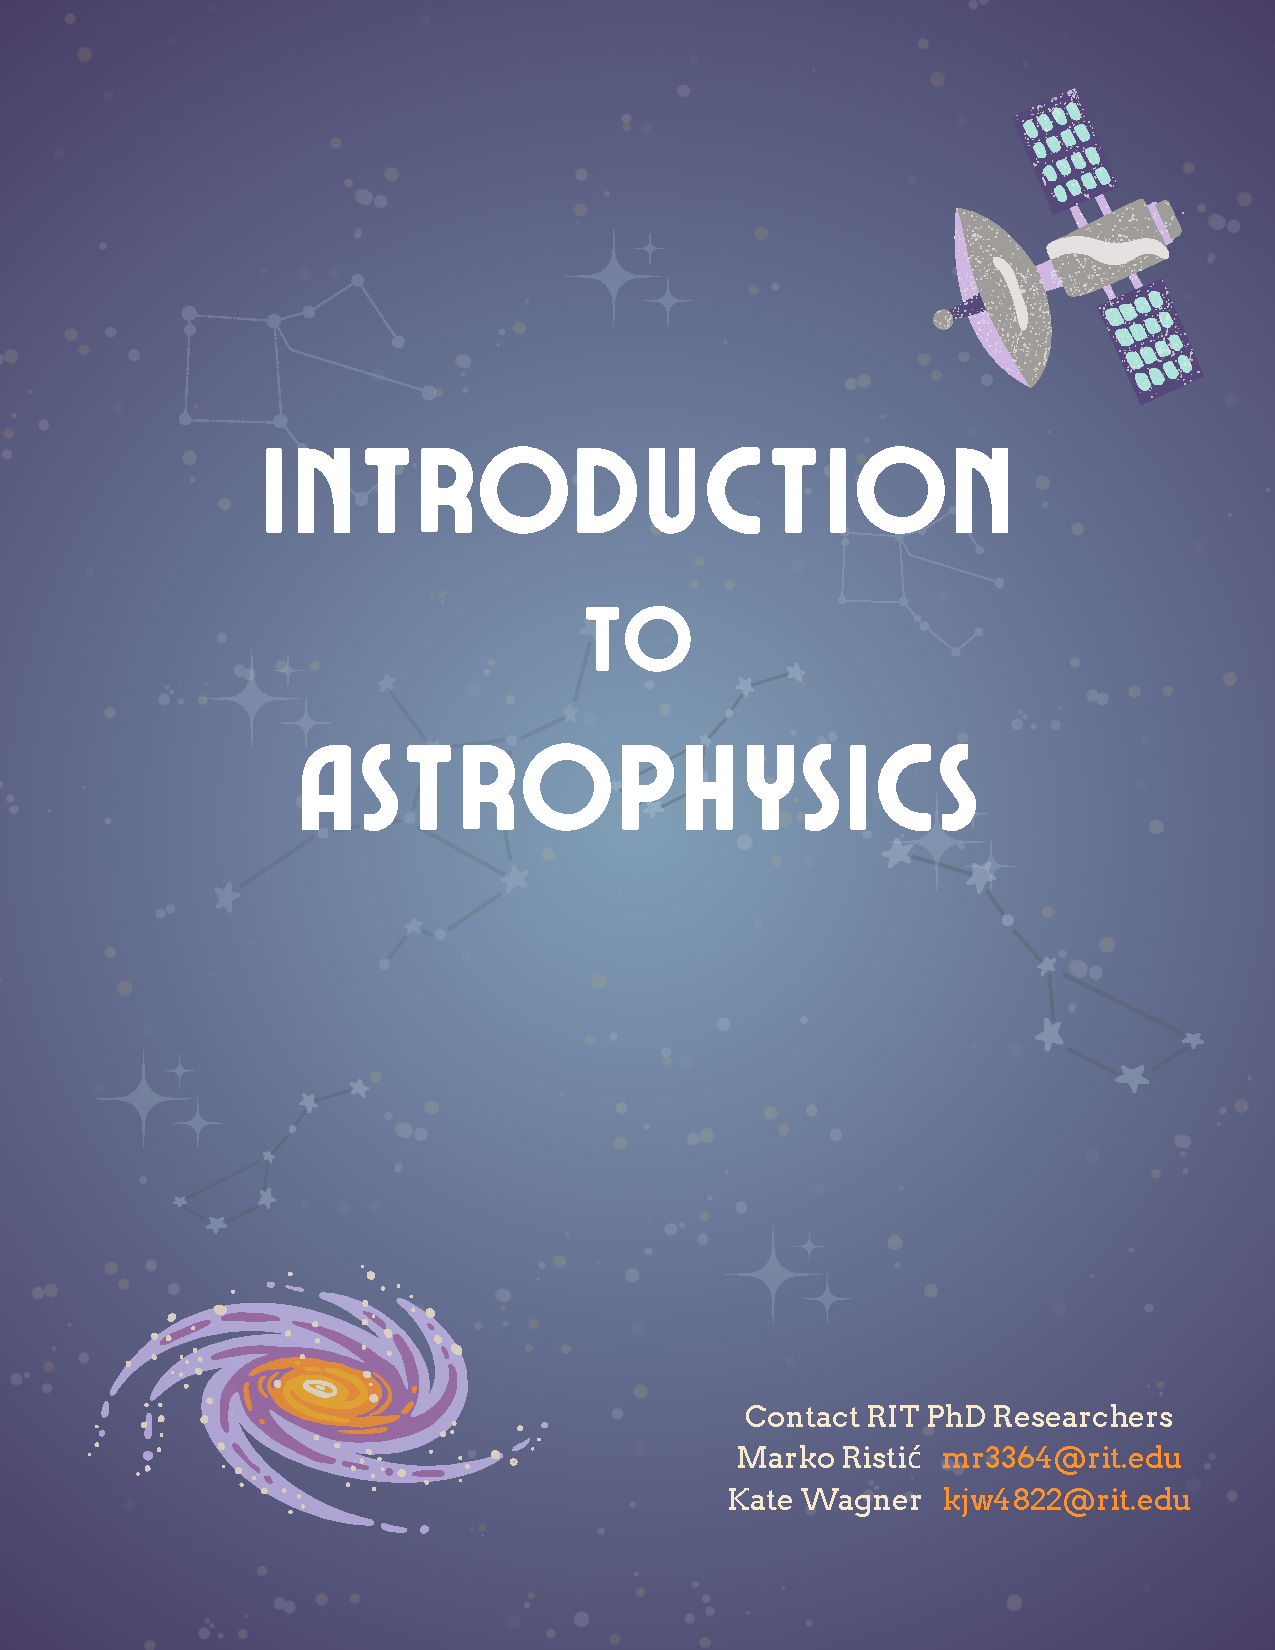
\includepdf{cover.pdf}

\clearpage

\maketitle

\section{Introduction}

Astronomy and astrophysics are more exciting than ever as technological and computational advances have allowed scientists to explore the Universe like never before. With this introductory computer lab, we hope to show you the basics of how the three main ``specializations" in astrophysics function. Astrophysical engineers build high-quality instruments which are capable of detecting signals from far-away stars and galaxies. Observers use these instruments to measure specific astrophysical objects or occurrences which they provide to theorists. Theorists create models which help explain the astrophysical nature of the observations. All three groups work together to try and understand the peculiar nature of our Universe. During today's lab, you will take on the role of an astrophysicist in each of these groups and do some investigative science of your own! We hope you enjoy your ``grand tour" of astrophysics!

\begin{figure}[hb!]
    \centering
    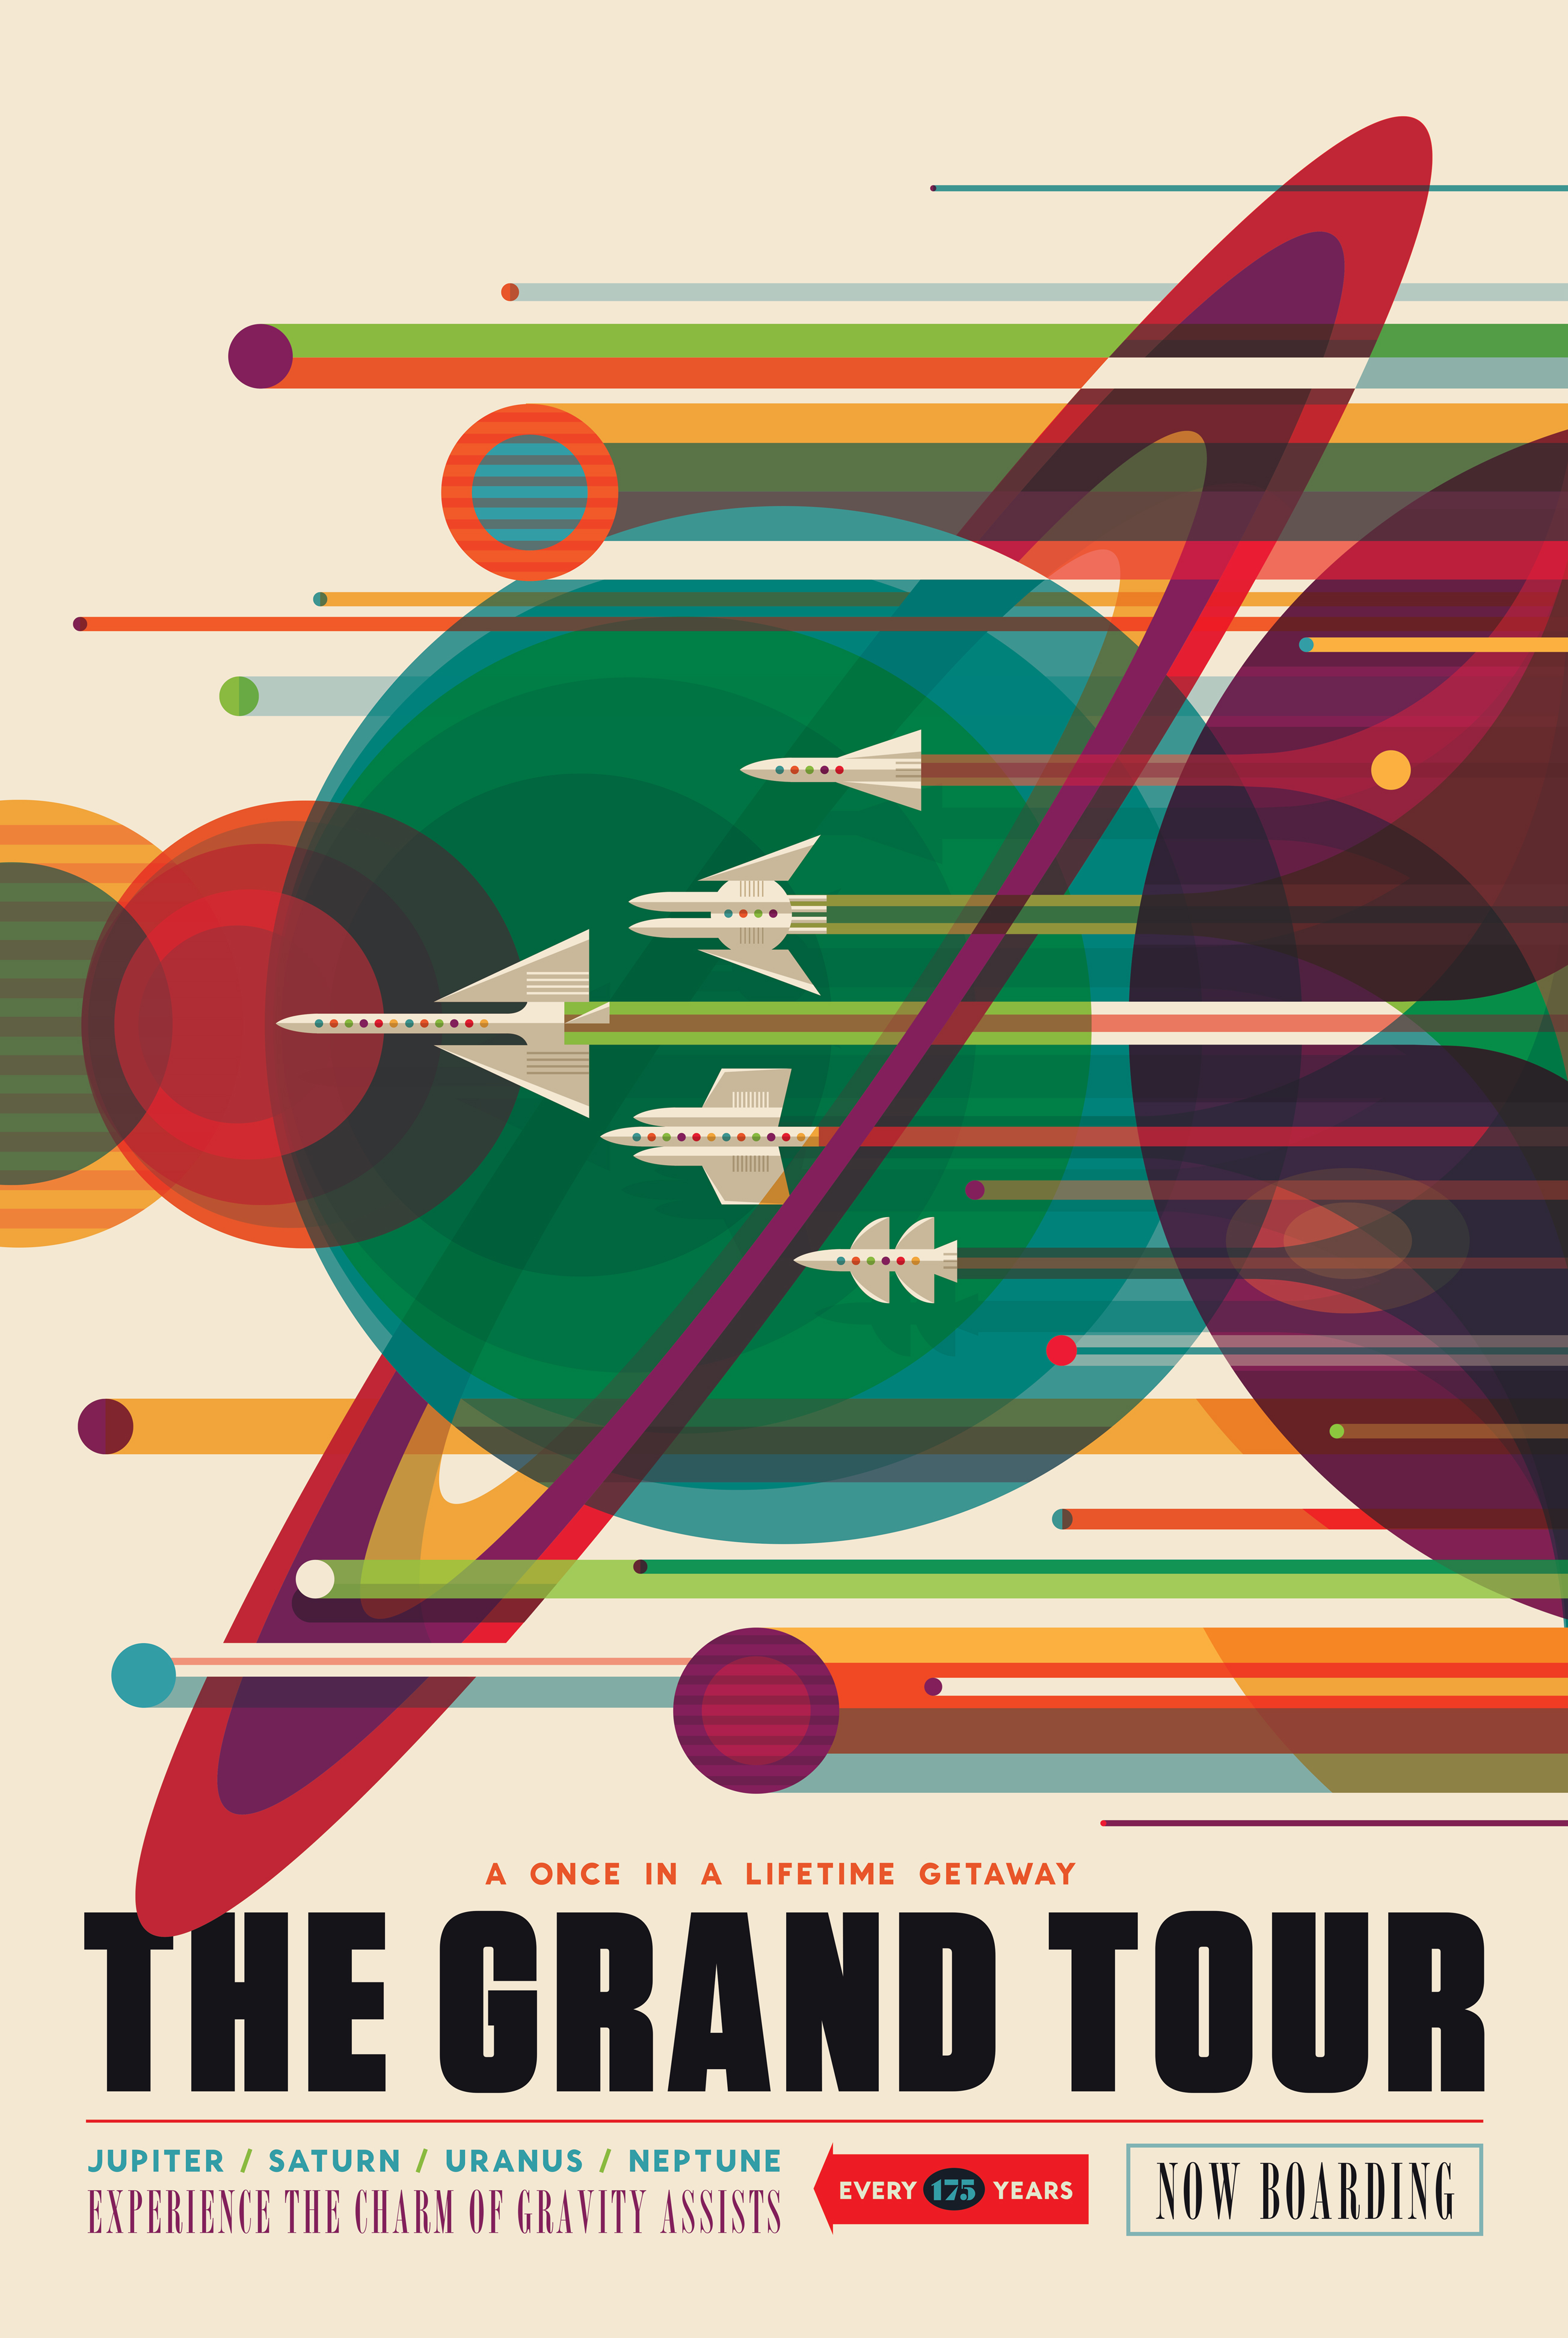
\includegraphics[width=.475\linewidth]{grand_tour.jpg}
    \caption{NASA space tourism poster of the Grand Tour of Jupyter, Saturn, Uranus, and Neptune. See more at \url{https://www.jpl.nasa.gov/galleries/visions-of-the-future}.}
    \label{fig:my_label}
\end{figure}

\newpage

\section{Observational Astrophysics}

%\kw{TO DO: Think about if it's too much to add a simple radius calculation to the code to add a classification component to the coding part of this module. Seems very doable. Need data for a couple more systems to have say 3 total.}

We live in an era of astronomy where space-based telescopes are extremely sensitive to distant sources of light. Satellite surveys like \textit{Kepler}, \textit{TESS}, and \textit{JWST} look at massive areas of the sky, collecting data all the time. This means scientists have an incredible amount of high quality data to use in order to make discoveries. Observational astrophysicists gather this data and make sense of it to make new discoveries.

\subsection{Observing Exoplanets}
When we look up into the night sky, we know most of the tiny dots of light we see are stars. There are thousands of them! On top of that, scientists think that most stars have planetary systems just like ours. Since satellite missions like \textit{TESS} and \textit{JWST} have such high sensitivity, scientists use this data to find evidence of planets around other stars. These are called \textbf{exoplanets}. The first exoplanets were found in the 1990s. Now, thousands of them have been discovered. There are four categories of exoplanet: Gas-giant, Neptunian, super-Earth, and terrestrial.

\begin{figure}[ht]
    \centering
    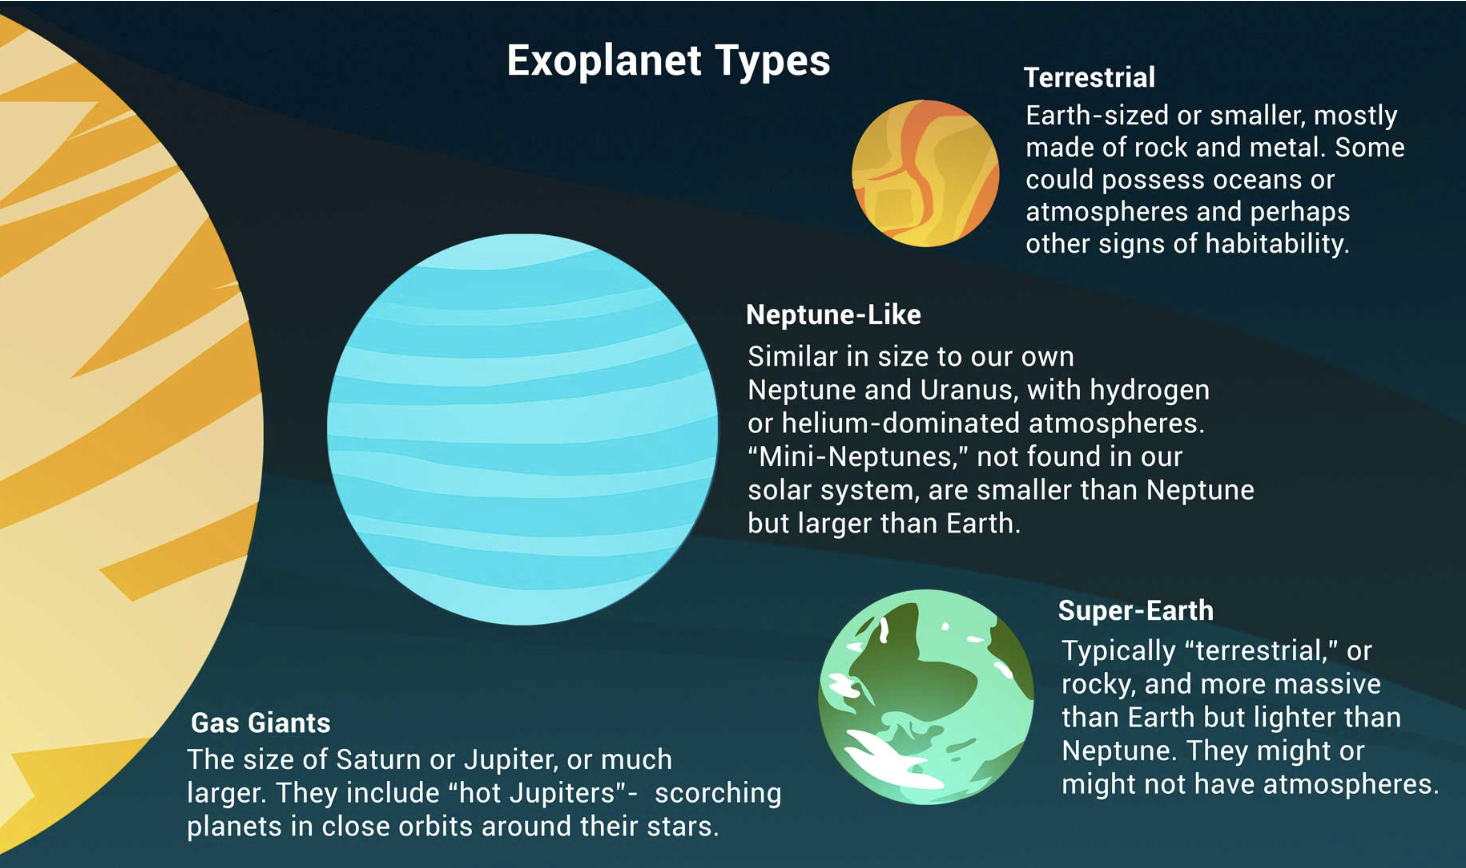
\includegraphics[width=\textwidth]{exo_types.png}
    \caption{Scientists observe a variety of types of exoplanets, and try to place them in categories based on their physical size and mass, the size of their orbit, and estimated temperature. (Credit: NASA/JPL-Caltech)}
    \label{fig:exo_types}
\end{figure}

\noindent Gas-giants are really large planets, the size of Saturn or Jupiter. These were some of the first exoplanets to be discovered. This makes sense, because of their larger size makes them easier to see to than other, smaller types. The planets orbit very close to their host stars, making them extremely hot. Next, Neptunian exoplanets are a bit smaller and have rocky interiors with hydrogen or helium-dominated atmospheres. These atmospheres can make it difficult to learn much about these planets from large distances for a variety of reasons. In another category, exoplanets classified as super-Earths are slightly larger than Earth, but not quite as big as Neptune. These exoplanets are pretty mysterious, because they are not like anything we see in our own solar system. Finally, terrestrial planets are Earth-sized and smaller. Scientists examine these exoplanets for signs of water and habitability. Very few terrestrial exoplanets have been discovered relative to the other types.

\newpage

\noindent Exoplanets are not usually observed in the same way you might look at the moon or Saturn through a telescope in your backyard. That type of observing is called \textbf{direct imaging}. Exoplanet science requires one of a variety of indirect observation methods. The most common indirect way to observe exoplanets is called the \textbf{transit method}. According to NASA, about 4000 exoplanets have been discovered using the transit method, whereas only about 60 have been directly imaged.
\\\\
\noindent How does the transit method actually work? A good analogy is a car's headlights on a dark street. Facing you, the car's headlights create a bright glow, and it is difficult to see other surrounding objects. However, when something passes in front of the headlights, the shape is illuminated from behind, blocking some of the bright light from the headlights. You can see how this might look in Figure \ref{fig:truck} This allows you to make out some information about the passing object. A large truck blocks a lot of the light, whereas a bicycle would block much less.

\begin{figure}[ht]
    \centering
    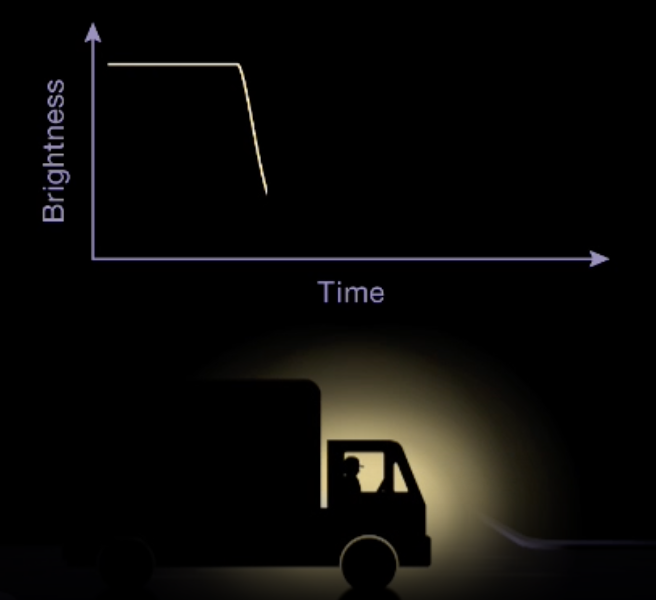
\includegraphics[width=0.5\textwidth]{headlights.png}
    \caption{A large truck blocks the some of the light from a car's headlights as it passes through an intersection. This allows the viewer to make out the passing truck, whereas before it passed in front of the headlights, it was obscured by the darkness. Watch the whole video \href{https://exoplanets.nasa.gov/resources/2338/exoplanet-detection-transit-method/}{here}! (Credit: NASA/JPL-Caltech)}
    \label{fig:truck}
\end{figure}

\noindent Scientists use a similar method of observing how much light is blocked by passing objects to deduce the existence of exoplanets. Space telescopes collect light from the stars they observe, recording the brightness over periods of time. Since planets orbit around their host stars, like Earth orbits around the Sun, an exoplanet eventually passes in front of the host star from the direction the space telescope is pointing. You can imagine a straight line between the telescope, the exoplanet, and the star. This passage causes the total brightness of the star to change just a tiny bit, as it becomes like a shadow crossing in front of the star while the telescope looks at it. This tiny dimming effect can be seen directly in the data the telescope records about the brightness of the star. It appears as a dip down in the total brightness of the star-planet system. Scientists called this total brightness \textbf{flux},  as you can see in Figure \ref{fig:exo_transit}.
\\\\
\noindent Two of the important quantities for scientists interested in learning about an exoplanet are \textbf{period} and \textbf{transit depth}. The measurement of the depth of the dip in total brightness is called the \textbf{transit depth}. The \textbf{period} is a measurement of how long it takes for the exoplanet to go all the way around the star, beginning and ending at the same location. During each period, there are two dips - one when the planet is in front of the star, blocking some of the stars light from reaching the telescope, and another when it goes behind the star, so it is no longer able to contribute to the star + planet brightness.

\newpage

\begin{figure}[ht]
    \centering
    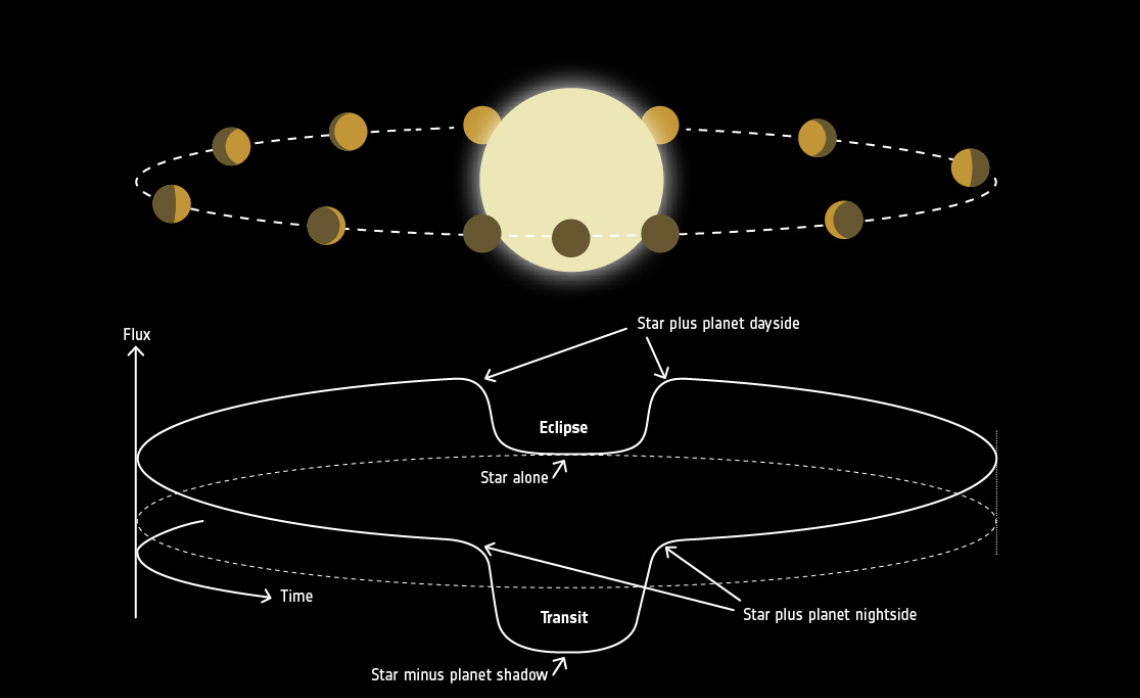
\includegraphics[width=\textwidth]{exo_transit.png}
    \caption{An exoplanet orbits its host star, and the total brightness of the system is tracked over time. When the planet is not directly in front of or behind the star, the total brightness is a sum of the light of the star and the light that illuminates the exoplanet. When the planet crosses in front of or behind the star, the total amount of light decreases by a very tiny, but measurable amount. (Credit: ESA)}
    \label{fig:exo_transit}
\end{figure}


\noindent Measuring the period and transit depth of these exoplanets gives us information about the mass and size of the planets. These measurements enable further science, including to figure out how much energy from the host star strikes the surface of the planet, allowing scientists to estimate things like temperature and color of the sky if you were standing on the surface.

\newpage

\subsection{Lab Instructions}
Now it's your turn to be an exoplanet scientist!

\subsection*{Introduction}
Start by opening up the \texttt{observational.ipynb} notebook file.
    \begin{enumerate}
    \item The code in the Jupyter notebooks is broken up into short boxes called \textbf{cells}. Each individual cell only runs the code inside of it.
    \item Any line of code that has \texttt{\#} symbols at the beginning of it is called a \textbf{comment}. Comments serve as human readable information to make code more user friendly, and are not evaluated as part of the program.
    \item Practice running the first cell in the notebook. You can run the cell by clicking on it so it's selected, and then clicking the ``Run" button in the menu bar. You may also use the ``Ctrl+Enter" shortcut.
    \item If you change code in the cells near the beginning, the output of later cells may be affected. It is best practice to rerun all the cells after the one you changed to make sure your outputs are correct.
    \end{enumerate}
In code notebooks or scripts, the user typically imports necessary code packages/libraries and script dependencies. This is what the first cell of your notebook does. Run this cell before continuing. If later you're interested in knowing more about importing, see Appendix \ref{a:packages}.

\subsection*{Exoplanet Data}
In the second cell, we begin by loading the data from an external file into the notebook so we can use and visualize it. If you were to open the file \texttt{`5651104/plot.tbl'}, you would see lots of columns of data. Alone, the columns of numbers do not mean a lot to us. 

\begin{figure}[hb!]
    \centering
    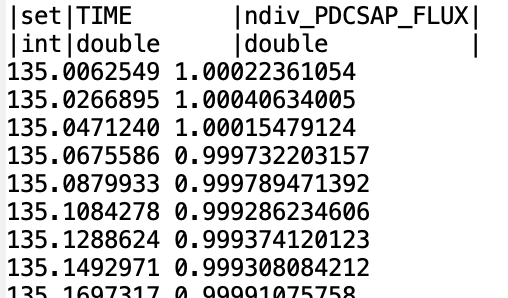
\includegraphics[width=.275\linewidth]{data_example.png}
    \caption{Screenshot of part of the file. It contains long lists of numbers that we need to make sense of.}
    \label{fig:data_example}
\end{figure}

\noindent Making plots to visualize data is very important for understanding the relationship between variables, which are \texttt{time} and \texttt{flux} in this case. We create a variable called \texttt{data} to hold all the contents of the file we are going to use.

\begin{enumerate}
    \item \texttt{time}: The first column of data from the external file gets defined in the \texttt{time} variable. You might notice that it is defined as \texttt{data[0]}. In programming, the first element of lists is generally labelled as the zeroeth element, rather than the first. So, reading in ``column 0" of the data gives us a list of what we think of as the first column in the file.
    \item \texttt{flux}: Next, \texttt{flux} holds the second column of data from the external file. Notice again that this column is accessed by writing \texttt{data[1]}, because first column is ``column 0". Remember from above that \textbf{flux} is like the total brightness of the system.
\end{enumerate}

\noindent Run the second cell. You should see a plot! This puts some of the data from the file into the plot showing the brightness data of the system plotted over time. This plot represents one exoplanet transit. You can see nice definition of the dip in brightness when the exoplanet is passing by the star.


\noindent Now run the third cell. Notice how the time scale on the bottom axis has changed as compared to the first plot. We are now looking at a zoomed out version of the beginning of the data from the first plot. Now you should be able to see two dips in the total brightness. This should remind you of Figure \ref{fig:exo_transit}. This plot shows one whole orbit of an exoplanet around its host star.
\\\\\
Run the next cell. This plot zooms out even further. Now at certain intervals there are large dips in the overall brightness. Do you notice that these dips appear on fairly regular intervals? Since the exoplanet is going around and around its host star at a regular rate, the system is \textbf{periodic}. This means that we can track the system over time and learn things about its regular behavior.

\subsection*{Making Sense of Light Curves}

\textbf{Investigate:} Remember that scientists want to measure the \textbf{period} of the exoplanet. The best way to do this is to measure the time between dips in the data. To the best of your ability, look at the plot you created and estimate the amount of time the dips. Click on \texttt{period\_estimate = } and type your best guess. Remove the \texttt{\#} symbol at the beginning of the line and run the cell.

\vspace{2mm}

\noindent The other important quantity scientists work hard to find is \textbf{transit depth}. This measures how much of a dip in the total brightness there is when an exoplanet crosses in front of the star.

\vspace{2mm}

\noindent You might notice that the dips have fewer points than the rest of your plot, where the points mostly stay around 1.0. To get a more accurate estimate of the transit depth, we can put slices of data on top of each other in a way that lines up the dips. This ``slicing and stacking" is called \textbf{folding}, and it combines all the knowledge of the dips over time to give a more accurate estimate of what the transit depth might be for this exoplanet.

\begin{figure}[hb!]
    \centering
    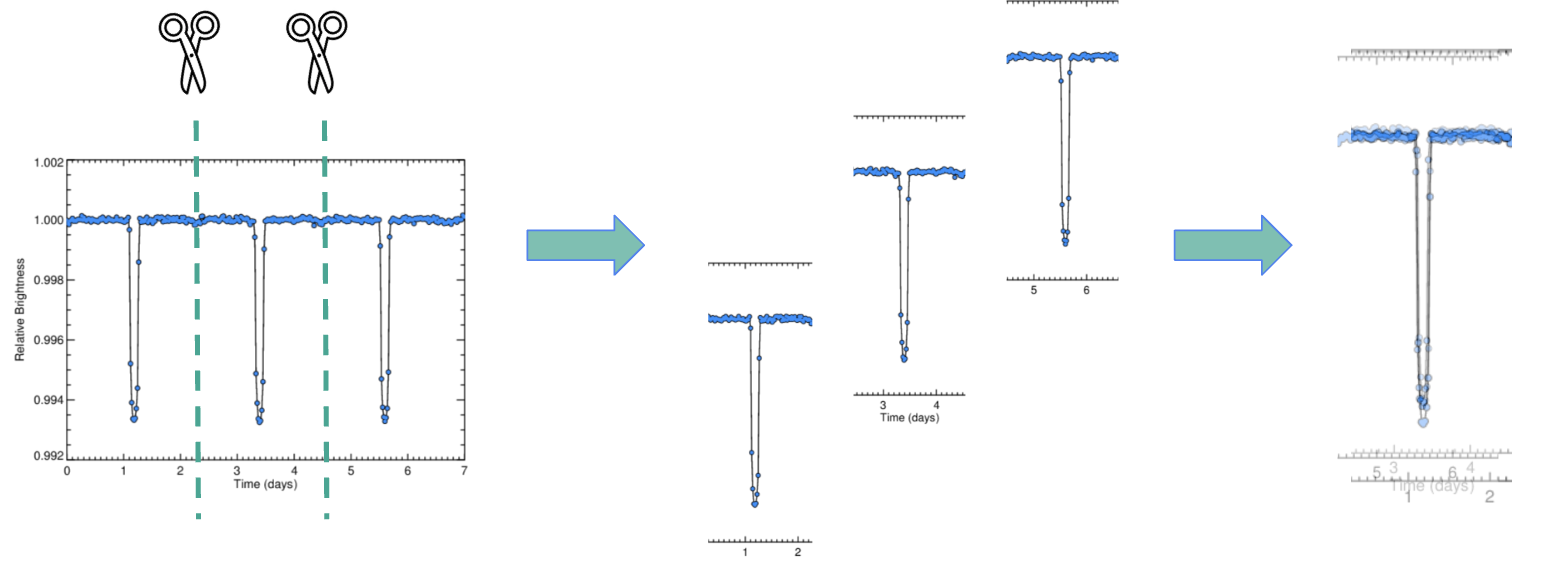
\includegraphics[width=0.8\textwidth]{folding_example.png}
    \caption{A diagram of how light curve data is folded. First, the original data is cut up into equal slices using information about the period to determine the slice size. Then the slices get stacked or folded on top of each other. More data samples means that measurements can be more accurate, so folding the light curve gives more information for better measurements of the data.}
    \label{fig:data_example}
\end{figure}

\noindent The folding size of the slices is determined by the \textbf{period}. We take slices that are the length of one half of the period (so that only one dip is included), and stack them up. This is why it's important to have an accurate measurement of the period!

\vspace{2mm}

\noindent Run the fourth cell. This cell performs the light curve \textbf{folding}. The data gets sliced up, stacked, and plotted. Now, all the dips are on top of each other and we have all the information about the dips in flux that is available from the data. This cell uses \textit{your} period estimate.

\vspace{2mm}

\noindent Now, run the fifth cell. This uses the \textit{real} value of the period to do the folding.

\vspace{2mm}

\noindent\textbf{Investigate:} What happens to the folded light curve when you use your estimate of the period versus when you use the known period of the exoplanet?

\subsection*{Using Light Curves to Learn}

Scientists use the folded light curves to find the \textbf{transit depth}. This allows them to find the size of the exoplanet.

\vspace{2mm}
    
\noindent \textbf{Investigate:} Using the folded light curve with the known period, estimate the amount that the brightness dips down. Enter your estimate in the fifth cell next to \texttt{depth = }, and again remove the \texttt{\#} from the beginning of the line. Run the cell.

\vspace{2mm}
  
\noindent \textbf{Investigate:} In the last cell, we are taking the transit depth and using a known relationship (see Appendix \ref{a:starsize} later if you are interested in a deeper explanation) to convert it into an estimate for the radius of the exoplanet. This cell prints out the size of the exoplanet in terms of how many times the radius of Earth this exoplanet is. What type of exoplanet would you classify this as?

\vspace{10mm}

\begin{table}[h]
\centering
\begin{tabular}{|c|c|}
\hline
Planet  & Size Relative to Earth \\ \hhline{|=|=|}
Mercury &   0.38   \\ \hline
Venus   &   0.95   \\ \hline
Earth   &   1.0    \\ \hline
Mars    &   0.53   \\ \hline
Jupiter &   11.0   \\ \hline
Saturn  &   9.0    \\ \hline
Uranus  &   4.0    \\ \hline
Neptune &   3.9    \\ \hline
\end{tabular}
\label{tab:sizes}
\caption{A table containing the sizes of the planets in the Solar System in terms of their relative size to Earth. Use this table to classify your exoplanet in one of the exoplanet type categories.}
\end{table}

\noindent The data for this module were obtained from the \href{https://exoplanetarchive.ipac.caltech.edu/overview/kepler-695b}{NASA Exoplanet Archive}.

\clearpage

\section{Theoretical Astrophysics}

%\kw{Describe what is ``theoretical" astronomy \& also make sure this is framed as theory and not just a \textit{different} kind of observation}

Theoretical astrophysics includes the use of mathematical and computational models created based on physics to describe astronomical systems. Where observation provides real data about how objects in space behave, theory connects that data together into a full understanding and allows scientists to make predictions about phenomena that haven’t yet been observed. These models are often then later applied to observational data.

\subsection{Studying Black Holes}

Black holes are mysterious and powerful objects in the Universe. Their mass is huge but their size is very compact. For example, a black hole that has one thousand times the mass of our sun is only about the size of the Earth. This means that gravity is extremely strong near black holes, so strong that nothing can escape - not even light.
\\\\
Where do black holes come from? They begin as ordinary stars. All the stars we see in the night sky are actively burning fuel and emitting light. Eventually, they burn through all their fuel and die. The process of dying can vary between stars, but some stars can leave behind a black hole when they die. If the original star had enough mass, all the stuff (gas, etc.) from the star explodes out into a giant cloud, but then collapses back in on itself to form a very small object - a black hole.
\\\\
Many stars in the Universe are not alone, unlike our Sun. Scientists observe many systems that have two stars, called \textbf{binary systems}, and some even three or more stars. For binaries, when both stars eventually die, it is possible that both turn into black holes. This means that two black holes can be bound together in an orbit, creating a \textbf{binary black hole}.

\begin{figure}[h]
    \centering
    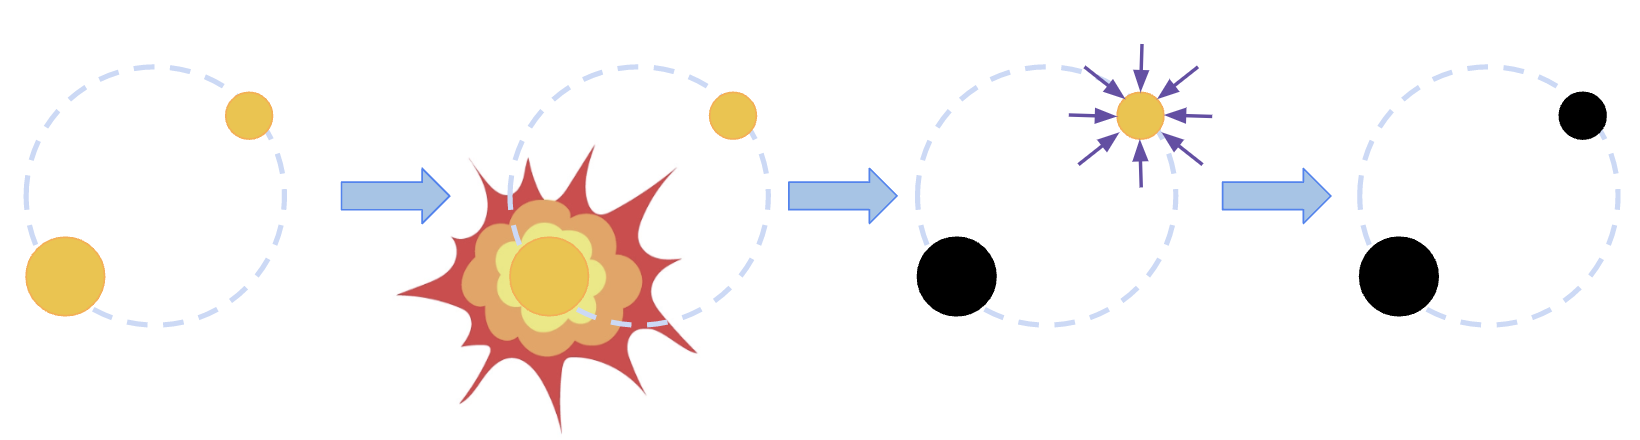
\includegraphics[width=0.75\textwidth]{bbh_formation.png}
    \caption{Oversimplified example formation process for a binary black hole system. Two stars in a binary evolve and die, turning a binary star system into a binary black hole.}
    \label{fig:bbh_form}
\end{figure}

\noindent Black holes exert such a strong gravitational pull on their surroundings that they can even trap light. This means we cannot observe black holes with the same telescopes we use for stars and galaxies. The telescopes you may be more familiar with observe electromagnetic light. For example, visible light that we can see with our eyes can be observed using standard telescopes. However, since black holes trap all the light, different detection methods needed to be developed in order to study these fascinating objects. \\

\begin{figure}[h]
    \centering
    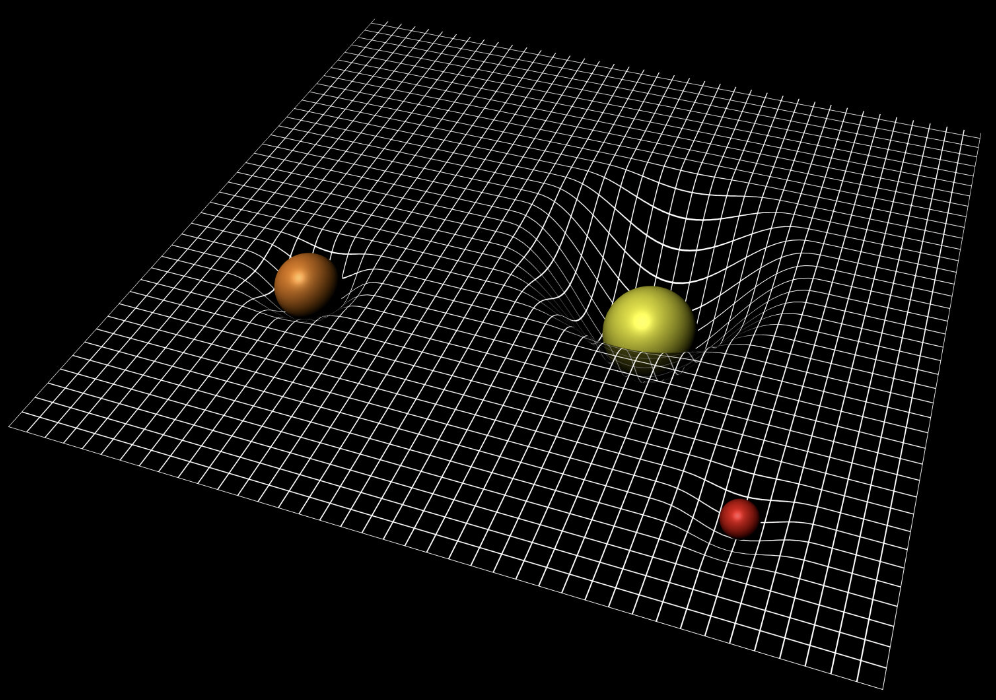
\includegraphics[width=0.45\textwidth]{spacetime.png}
    \caption{Heavy (massive) objects create impressions on spacetime, causing curvature nearby.The more curvature an object creates, the more gravity it has. (Credit: ESA)}
    \label{fig:spacetime}
\end{figure}

%\newpage

\noindent In 1916, Albert Einstein wrote about the idea of space and time being combined together as if they were a fabric that all the objects in the Universe rest on. He theorized that objects with more mass would create larger impressions on this invisible fabric of the Universe, such as in Figure \ref{fig:spacetime}. Then, the amount of gravity an object has is related to how much curvature it creates in the surrounding space-time fabric. The size of the impact an object has on space-time is related to how much gravity it has.
\\\\
\noindent When extremely massive objects, like black holes, orbit around each other, these gravitational impressions also move. As the objects circle around each other, the movement causes a ripple effect that travels across the spacetime fabric. Scientists call these \textbf{gravitational waves}, because the waves are caused by changes in the fabric of spacetime due to objects' gravity. The ripples that move outward, just like ripples in a pond created when you throw a stone onto the surface, but gravitational waves travel at the speed of light.
\\\\
As gravitational waves travel, they stretch and compress spacetime. If you imagine a grid of isolated particles at rest in spacetime, when a gravitational wave or a massive object passes through the grid, the distances between particles gets shorter and longer in a periodic pattern. The change in the distance between particles is called the gravitational wave \textbf{strain}.

\begin{figure}[h]
    \centering
    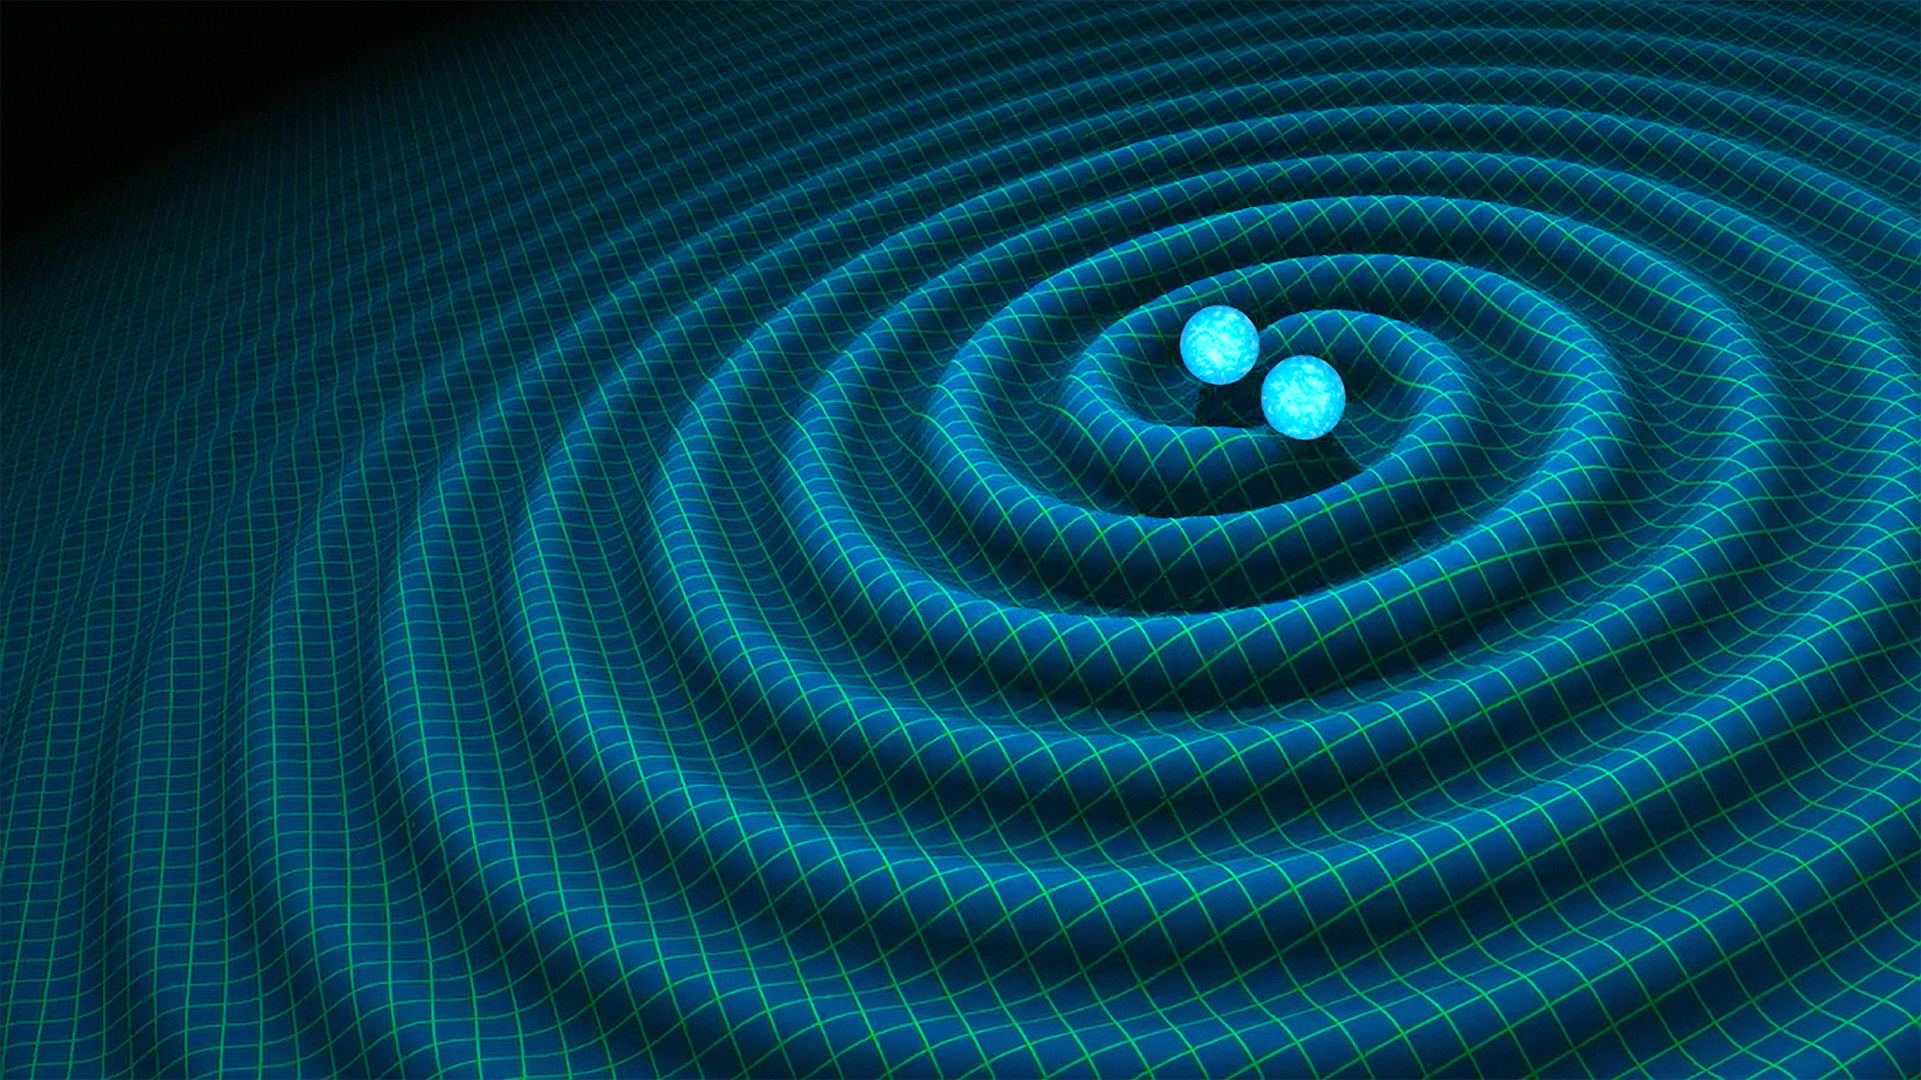
\includegraphics[width=0.7\textwidth]{spacetime_bbh.jpeg}
    \caption{Two extremely massive objects spiral around each other, bound to eventually collide and merge. As the spiral in, the curvature they impart on spacetime moves with them. The impressions created by their movements are called gravitational waves, and they are detected on Earth. (Credit: NASA)}
    \label{fig:spacetime_bbh}
\end{figure}

\noindent It is important to note that gravitational waves don't just affect particles that are close together - they stretch and compress the fabric of space-time itself, affecting objects that are separated by vast distances. However, gravitational waves are very weak. Typically, the gravitational wave strain produces an effect smaller than the size of the nucleus of an atom. This makes gravitational waves incredibly difficult to detect, which is why it took about one hundred years after Einstein published his theory of general relativity for gravitational waves to be detected for the first time.
\\\\
To measure the expansion and contraction of spacetime, scientists built detectors like LIGO and others (Virgo, KAGRA, etc). The LIGO
detector uses lasers to measure how much the spacetime distance changed due to gravitational waves from the black holes smashing into each other.\\

\begin{figure}[h]
    \centering
    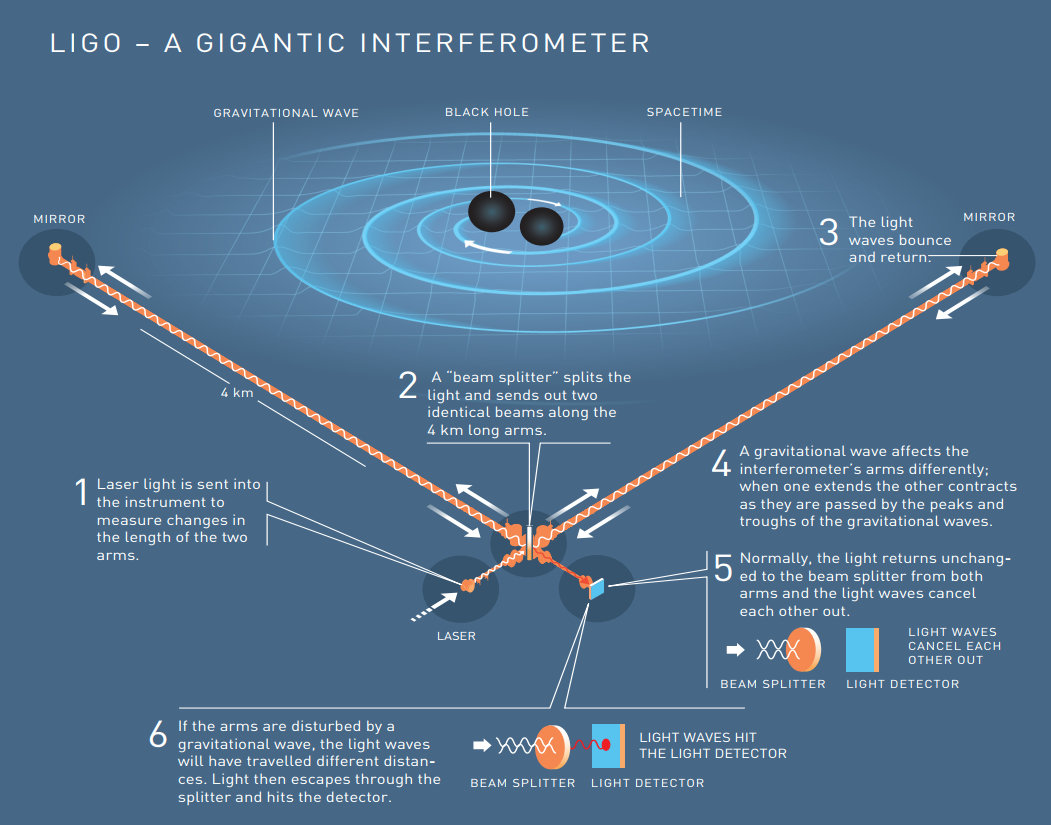
\includegraphics[width=\textwidth]{ligo.jpeg}
    \caption{Read figure blurbs carefully if you are interested in the details of the LIGO detector. Each step ealks through the process of using this complex detector to collect data that contains gravitational wave signals. (Credit: MIT)}
    \label{fig:ligo}
\end{figure}

\noindent The shape of the waves tells scientists certain  information about the black holes they came from. This information travels with the gravitational waves, all the way to Earth. Scientists analyze the shape of the waves to learn about the masses of the black holes and how far away from us they were when the merged together.
\\\\
When a gravitational wave passes through an interferometer like LIGO, it causes the lengths of the two arms of the interferometer to change slightly. By measuring these changes in length, scientists can infer the presence of a gravitational wave. As mentioned above, the strength of a gravitational wave is usually measured in terms of its \textbf{strain}. 
\\\\
The strain or strength of a gravitational wave is extremely small, but now LIGO is sensitive enough to these tiny perturbations that scientists can use information from those patterns on the photodectector to determine intrinsic properties of the systems. These
quantities include mass and distance. 
\\\\
The \textbf{strain} is directly proportional to the black hole masses, meaning that larger masses create larger gravitational wave strain. The strain in inversely proportional to the distance to the binary. If the binary is far away, the signal is much weaker than if it were moved closer to Earth. Keep this in mind as you begin your gravitational wave investigation!


% For simplicity, consider that the gravitational wave strain $h$ may be approximated as:

% $$
% h \sim \frac{GM}{c^2}\times \frac{1}{r}\times \bigg(\frac{v}{c}\bigg)^2,
% $$

% where $G$ and $c$ are the gravitational constant and the speed of light, $M$ is the black hole mass, $v$ is the speeds of the masses, and $r$ is the distance away from us the system is.

\newpage

\subsection{Lab Instructions}
Now it's your turn to be a gravitational wave investigator!
\subsection*{Introduction}
Start by opening up the \texttt{theoretical.ipynb} notebook file.
    \begin{enumerate}
    \item The code in the Jupyter notebooks is broken up into short boxes called \textbf{cells}. Each individual cell only runs the code inside of it.
    \item Any line of code that has \texttt{\#} symbols at the beginning of it is called a \textbf{comment}. Comments serve as human readable information to make code more user friendly, and are not evaluated as part of the program.
    \item Practice running the first cell in the notebook. You can run the cell by clicking on it so it's selected, and then clicking the ``Run" button in the menu bar. You may also use the ``Ctrl+Enter" shortcut.
    \item If you change code in the cells near the beginning, the output of later cells may be affected. It is best practice to rerun all the cells after the one you changed to make sure your outputs are correct.
    \end{enumerate}
In code notebooks or scripts, the user typically imports necessary code packages/libraries and script dependencies. This is what the first cell of your notebook does. Run this cell before continuing. If later you're interested in knowing more about importing, see Appendix \ref{a:packages}.

\subsection*{Make a Signal}

First, let's take a look at some real data that LIGO collected. The second cell plots real gravitational wave data collected in the seconds surrounding LIGO's very first detection of gravitational waves. This occurred on September 14, 2015 (hence GW150914). It looks a little wobbly, but you can see the expected shape of a gravitational wave signal right there on your plot! Comparing the plot you made to Figure \ref{fig:imr}, you should be able to identify the inspiral, merger, and ringdown. 
\\\\\
\noindent Note that this is not exactly what the data looks like straight from the detector. Some signal processing has been performed. See Appendix \ref{a:sigproc} later if you are interested in a deeper explanation of this data was processed. 

\begin{figure}[h]
    \centering
    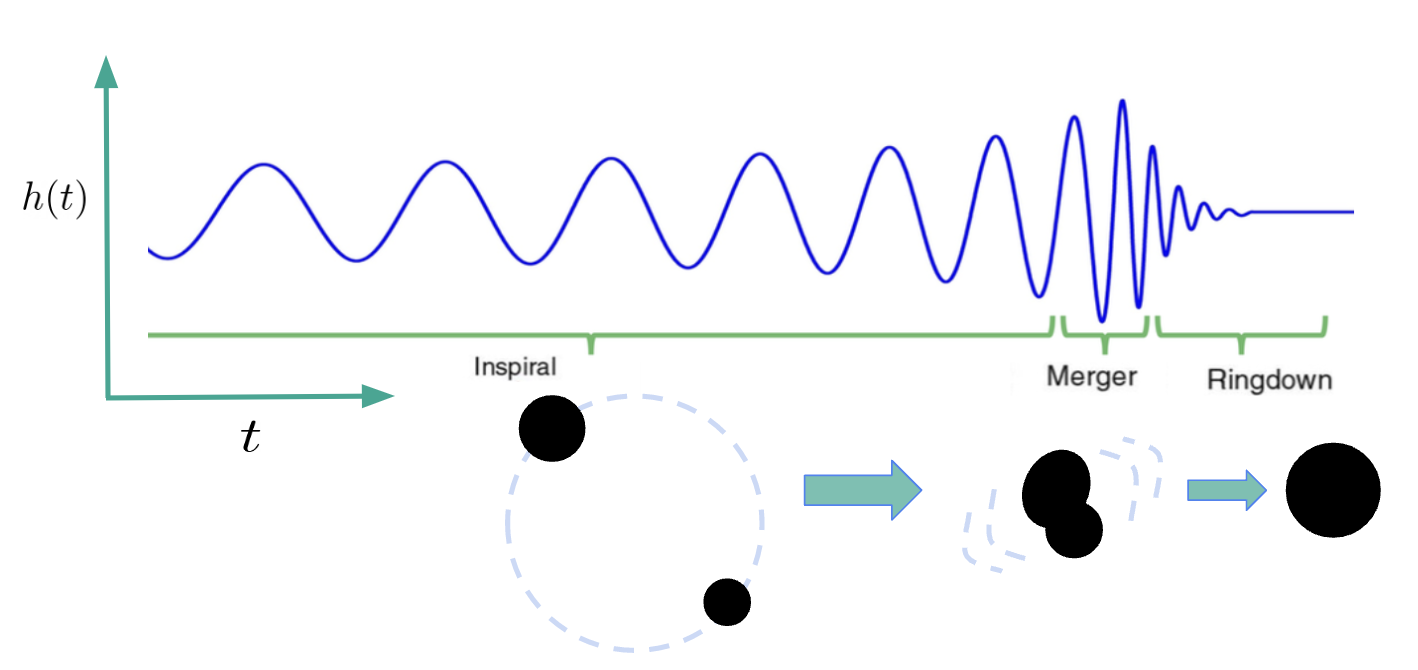
\includegraphics[width=0.8\textwidth]{imr.png}
    \caption{In the plot you can see each stage of the merger. You can see the \textbf{inspiral} as the height of the signal grows. The black holes \textbf{merge} at the largest peak and immediately the GW signal goes almost to zero. The \textbf{ringdown} is seen as the peaks are suddenly smaller, and eventually go back to zero.}
    \label{fig:imr}
\end{figure}

\noindent Next, astronomers fit theoretical models to their real data to investigate what type of binary black hole could have produced such a signal. To do this, we must create a signal model to place over the data. The third cell  defines some necessary variables, which here are the masses of your two black holes and the distance away from Earth the system is located. Run it. This saves those values so that they can be accessed as needed later. You will eventually try changing these values to see what happens!

\vspace{2mm}

\noindent The fourth cell then creates two black hole objects (\texttt{bh1} and \texttt{bh2}) at some distance away and makes them into a binary. For the black hole system, gravitational waves will only be observed if there are two black holes spiralling around each other. Then, the cell plots the gravitational wave signal we would see if there was a binary black hole with the particular mass and distance that was set. The height of the peaks in strain (y-axis) is called the \textbf{amplitude}. We call signals with larger amplitudes (higher peaks) \textbf{louder} signals.

\subsection*{Comparing Signals}
\noindent \textbf{Investigate:} Now that you have seen an example signal, try changing the masses of the two black holes to see what happens.
\\\\\
\textbf{\textit{NOTE: }}Each time you change the values in the third cell, you must also rerun the fourth cell so that the gravitational wave signal plot actually changes to reflect the new values you entered.

\begin{enumerate}

    \item What does the signal look like when the black holes have similar or the same mass?
    \questionspace
    
    \item What happens if you make the masses really large?
    \questionspace
    
    \item What happens if you make the masses really different from each other?
    \questionspace
    
    \item What happens if you make the distance large (i.e. far away)?
    \questionspace

\end{enumerate}

\noindent Now you have experience making model gravitational wave signals, and you understand the effect of changing the masses and distance on the shape and amplitude of the gravitational wave signal. Let's revisit the real data and put this all together. Try changing the values in the third cell, then running the fourth and fifth cells. The fifth cell shows your signal model on top of the real LIGO data!
\\\\\
\noindent \textbf{Investigate:} What values for \texttt{blackHole1\_mass}, \texttt{blackHole2\_mass}, and \texttt{system\_distance} create a signal that lines up with the shape of the real data? 
\vspace{5mm}
\begin{itemize}
    \item \texttt{blackHole1\_mass}:
    \item \texttt{blackHole2\_mass}:
    \item \texttt{system\_distance}:
\end{itemize}
\vspace{5mm}

\noindent This process is a simplified version of exactly what astronomers did when the first gravitational wave event was detected in 2015. The masses and distance you find approximately match the \textit{real} values of \textit{real} black hole merger event!

\clearpage

\section{Astronomical Instrumentation}

Astronomical instrumentation involves building high-technology cameras and other instruments that are used with large telescopes. Telescopes focus the light, and the instruments turn that light into data that scientists can make sense of. Learning about the universe requires the right tools, so developing instrumentation is an essential part of astronomical research.

\subsection{Background}

If you have ever looked up at the night sky, you have probably noticed that it's not empty. With your naked eye, you can easily see the Moon and some of the brightest or nearest stars in our Galaxy. To observe more distant stars, or even other galaxies, you would need to use a telescope. Suppose you have a fancy new telescope and find a cool galaxy that you want to show off to friends and family. How do you ``take a picture" of it?
\\\\
Telescopes essentially use fancy cameras, similar to the ones in smartphones, to capture the light from objects in space. Your telescope would start the process of taking a picture of the galaxy you are observing by receiving light from the galaxy. Without getting too complicated, we can measure the energy of light because it travels in a packet of energy called a ``photon." Each photon leaving the galaxy carries a certain amount of energy. When they get to Earth, the photons from the galaxy interact with the detector in the telescope via the \textbf{photovoltaic effect}. 
\begin{figure}[hb!]
    \centering
    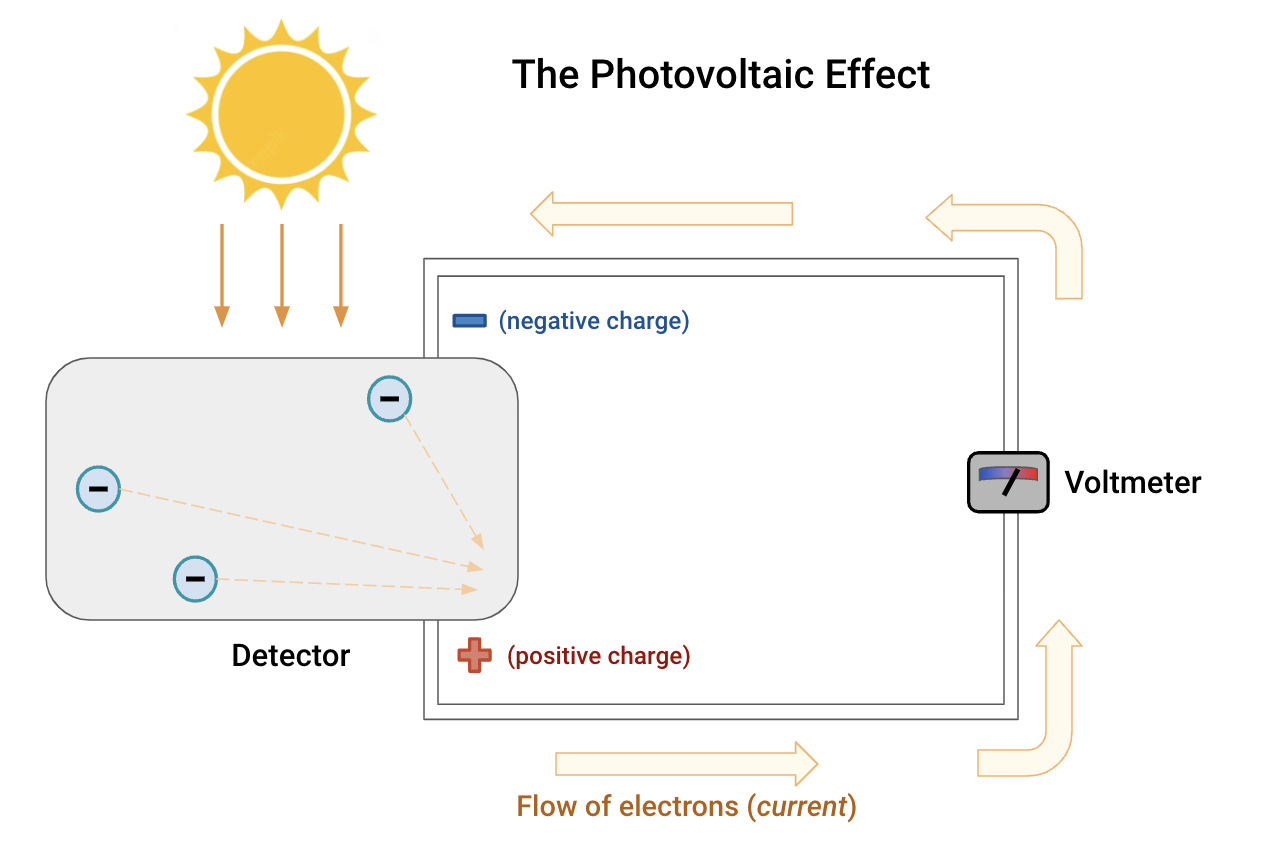
\includegraphics[width=.8\linewidth]{photovoltaic.png}
    \caption{Diagram of the photovoltaic effect. Light from a star (or other space object) interacts with the detector, freeing some electrons within the material. The electrons flow toward the positive charge and through the circuit on the right-hand side of the diagram. As they flow through the circuit, the electrons pass through a voltmeter. The voltage reported by the voltmeter is directly tied to how much light the detector received. This gives a direct connection between light energy (brightness or luminosity) and voltage.}
    \label{fig:photovoltaic}
\end{figure}
\\\\
The photovoltaic effect is a physical process in which the interaction of light with specific materials allows previously stationary electrons to move around freely. Once electrons have been freed by the interaction with light, a positive charge is turned on at one end of the material. The positive charge creates a circuit which guides the electrons from an area of higher concentration to an area of lower concentration. As these electrons flow toward the positive charge and through the circuit, they pass through a \textbf{voltmeter} which records their \textbf{voltage}.
%As the electrons move toward the positive charge, they generate an electric current which can be measured. 
This measured voltage is directly tied to the number of electrons. The number of electrons is in turn dependent on the energy of the packet of light observed. Simply put, the more energy we see from the observed galaxy, the higher the measured voltage is. As such, we can determine the brightness of the observed galaxy! 
\\\\
The detector consists of individual pixels which combine together to create an image. This is very similar to how individual pixels in a laptop screen work together to create the whole display. The process of measuring the energy of light happens in these individual pixels across the entire detector. The final image of the galaxy is made by combining the energy of light measured in each pixel in the detector grid. Figure \ref{fig:resolution} shows how increasing the number of pixels in the pixel grid increases the visual clarity of the final image. Finer features in the galaxy become clearer as more pixels are present in the detector. 
\\\\
Consider first the case of the 13x13 pixel grid (left-most image in Figure~\ref{fig:resolution}), where the center-most 3x3 square is yellow (or, in our galaxy analogy, bright), and the outer rim is blue (or, in our galaxy analogy, dark). At a low \textbf{resolution} of 13x13, it is hard to tell what the object being imaged is; for all we know, this could be a star! But, there is a clear distinction between the high-energy, bright, yellow region and the low-energy, dark, blue region. When the resolution is increased, it is clear that the image is of a galaxy, not a star. The finer features, like clumps of stars, also begin to become apparent at higher resolution.

\begin{figure}[ht!]
    \centering
    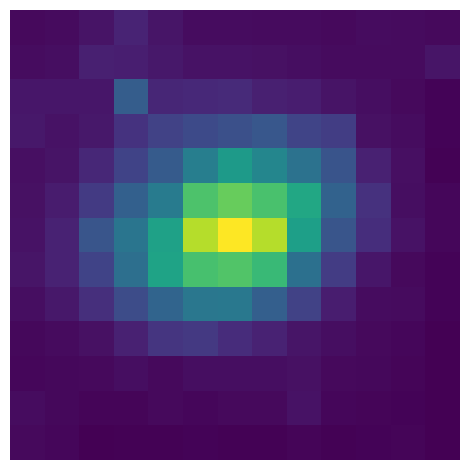
\includegraphics[width=0.23\linewidth]{galaxy_100.png}
    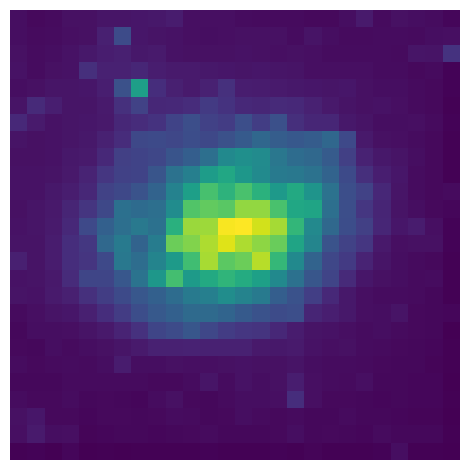
\includegraphics[width=0.23\linewidth]{galaxy_50.png}
    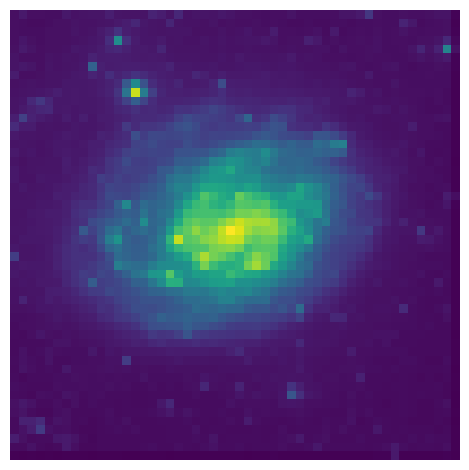
\includegraphics[width=0.23\linewidth]{galaxy_25.png}
    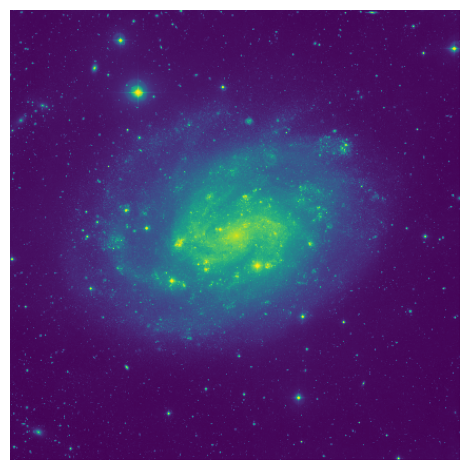
\includegraphics[width=0.23\linewidth]{galaxy_3.png}
    \caption{Example showing how the clarity of the galaxy increases as the number of pixels used to generate the image is also increased. The image resolutions are 13x13, 26x26, 52x52, and 427x427 from left to right.}
    \label{fig:resolution}
\end{figure}

\clearpage

\subsection{Lab Instructions}

For the instrumentation module, you will create your own simulated images of stars and galaxies. You will see for yourself how modifying the properties of your simulated detector affects your images. 

\subsubsection{Starting Off}

\begin{enumerate}
    \item Your laptop should be showing a block with code in it. If your laptop is instead showing a list of files with one being \texttt{instrumentation.ipynb}, ask an instructor for assistance.
        \begin{enumerate}
        \item The code in the Jupyter notebooks is broken up into cells, where each individual cell only runs the code inside of it.
        \item Each line of code in each cell can be easily identified by line numbers. If they are not already on, turn on line numbers via the menu at the top of the page. Click the third column, \texttt{View}, and then choose \texttt{Toggle Line Numbers}.
        \item Test your code by running the first cell in the notebook. You can run the cell by clicking on it and clicking the "Run" button in the menu bar or by using the "Ctrl+Enter" shortcut. Running the cell will display a real image of the ``Deep Field" taken by the recently launched JWST telescope.
        \end{enumerate}
\end{enumerate}

\subsubsection{Your First Image}

\begin{enumerate}
    \item Running the code cell displayed an image. But, what actually happened, and how did the code in the cell produce the image? 
    \item Line 1 simply tells the code to produce the plots under your code cell.
    \item Line 4 imports our \texttt{image} module which we will use to create the simulated image effects later on in the module. If later you're interested in knowing more about importing, see Appendix \ref{a:packages}.
    \item Line 9 defines the size of our pixel grid. A good starting point is an image with 1024x1024 pixels, which is defined in the Jupyter notebook on Line 9 as \texttt{image = img.Image(1024)}. This creates an ``image" variable and sets it to have 1024 pixels along each side. This grid of 1024x1024 pixels is how we are representing the "detector"!
%    \item Line 11 adds some objects - a mix of galaxies and stars! For a 1024x1024 pixel grid, we can comfortably add 25 objects without expecting too much overlap. This is done via \texttt{image.add\_objects(25, prob=0.3)} on Line 11. You will examine what the \texttt{prob} argument does in the next section. For now, leave it as-is.
    \item For now, ignore any image effects, leaving Lines 13 and 14 commented out. Commented lines are denoted by a \texttt{\#} at the front and they do not execute the code that follows the \texttt{\#} symbol. In the future, to uncomment a line, simply delete the \texttt{\#} symbol from the start of the Line. We will examine image effects shortly.
    \item Line 17 plots the image, which is the most important part of seeing your observations! This is done with the \texttt{image.plot()} command and is what produces the beautiful Deep Field image full of galaxies and stars.
    \item \textbf{Investigate:} Which objects in the Deep Field image do you think are stars and which are galaxies? How can you tell? Do all the stars look the same? Do all the galaxies look the same?
\end{enumerate}

\questionspace

%\subsubsection{The Fraction of Stars vs. Galaxies}

%\begin{enumerate}
%    \item At the end of the last section, you identified some stars and some galaxies. The number of each was determined by the \texttt{prob=0.3} argument in the \texttt{add\_objects} function on Line 11. In nature, the number of stars and galaxies is fixed, but with this code, you can modify your image to produce different results. Try changing the values provided to the \texttt{prob} argument, between 0 and 1, to figure out how the values for \texttt{prob} affect your image. \textbf{Don't forget to run the cell every time you want to run the code with a new modification!}
%    \item \textbf{Investigate:} What can you conclude about changes in the image as the value for \texttt{prob} is lower? What about when it is higher?
%\end{enumerate}

%\questionspace

\subsubsection{Adding Image Effects}

\begin{enumerate}
    \item When taking a real image with a detector, there will typically be some kind of impurity with the raw image. In this section, you will simulate some of the image effects which could happen.
    \item Here is the list of image effects we will consider, as well as their variable names for coding purposes (include the quotes!):
    \begin{enumerate}
        \item[$\smallcircle$] Dark Current: \texttt{"satellite\_transits"}
        \item[$\smallcircle$] Telescope Cover: \texttt{"telescope\_cover"}
        \item[$\smallcircle$] Dead Pixels: \texttt{"dead\_pixels"}
        \item[$\smallcircle$] Dead Arrays: \texttt{"dead\_arrays"}
        \item[$\smallcircle$] Cosmic Rays: \texttt{"cosmic\_rays"}
    \end{enumerate}
    \item \textbf{Investigate:} Before you begin, take a second to think about what each of these effects might do to the image. If you have no idea what an effect might do, take a wild guess and see if you were right later! \questionspace

    \item Start by uncommenting Line 14. This will implement the \texttt{satellite\_transits} effect. Note the formatting of \texttt{add\_effects(["satellite\_transits"])}, carefully considering the location of the parentheses \texttt{()}, brackets \texttt{[]}, and quotations \texttt{""} around the effect name. Line 13 (commented) shows a list of all applicable effects and the proper syntax to apply them, which you can use throughout the module.
    \item Try each effect one at a time, replacing the effect name in quotes with the variable names listed in Line 13 above. 
    \subitem \textbf{Hint:} For the \texttt{dead\_pixels} and \texttt{dead\_arrays} effects, it might be easier to see the effects on the image by reducing the number of pixels in the original image definition from 1024 to something smaller (512, 256, 128, etc.).
%    \subitem \textbf{Hint:} For the \texttt{dark\_current} effect, it may not be obvious at first glance what the difference is. Try comparing an image with the dark current effect to an image with \textbf{no effects applied}. Remember, to remove effects, comment out any lines with \texttt{image.add\_effects(...)} by putting a ``\#" at the start of the line. When comparing the images, hover your mouse over the area between the stars/galaxies. What do you notice for the values in the bottom-right corner of the image, to the right of the x- and y-coordinate values, for the images with and without dark current?
    \item \textbf{Investigate:} After having gone through each effect, what can you say about what they do to the image? How many of your initial guesses were right?
    \questionspace
    
\end{enumerate}

\subsubsection{Bonus: Sandbox Mode}

\begin{enumerate}
    \item At this point, you've gotten the hang of manipulating the image in various ways: adding image effects, examining how they change the quality of your image, and resizing the pixel grid. With the remaining time, feel free to combine all of these together to make whatever image you want! 
    \item This is your chance to have fun and really play around with the code. When playing with the pixel grid size, \textbf{keep the pixel grid size at or under 4096}!
    \item One suggestion could be a really high-resolution image using 4096x4096 pixels with no image effects! Instead of adding effects to worsen the image, see what cool details you can find by looking at the highest-resolution version.
    \item Alternatively, you could try to make a really bad-quality image, with a low-resolution 128x128 pixel grid, and some dead pixels/arrays. Then, see how many stars and galaxies you can actually make out in the that image!
    \item \textbf{Investigate:} What image did you create and how did it come out? What was expected and what was unexpected with your created image? 
    \questionspace
    
\end{enumerate}

\clearpage

\appendix

\section{Introductory Code Information}
\subsection{Importing Packages}
\label{a:packages}
Code packages/libraries and script dependencies are code files that contain useful pieces of code that might be used more than once. The pieces of code are also often more generic and can be used in a variety of applications. For example, in the observational notebook the first cell imports a script called \texttt{lightcurve}. This file contains functions to perform the core activities for the user in the background.
\\\\
In Python, we ask the notebook to look for  and read a script using the \texttt{\textcolor{green}{import}} command so that the user can actually use the contents of the script. Sometimes, packages have long names that are inconvenient to type over and over, so the user can temporarily rename the package for use in the script using the \texttt{\textcolor{Cerulean}{as}} command. So, we \texttt{\textcolor{green}{import}} the script \texttt{lightcurve} \texttt{\textcolor{Cerulean}{as}} \texttt{lc}.
\\\\
In the theoretical notebook, the first cell imports a script called \texttt{make\_waveform}. This file contains functions to perform the core activities for the user in the background. In Python, we ask the notebook to look for the script using the \texttt{\textcolor{magenta}{from}} command. We then use the \texttt{\textcolor{green}{import}} command to ask Python to read the script so that the user can actually use the contents of the script. So, \texttt{\textcolor{magenta}{from}} \texttt{make\_waveform}, we \texttt{\textcolor{green}{import}} everything, where \textbf{*} indicates that we are requesting that Python gives us access to all of the contents of the script.
\\\\
In this case, the author of the notebook knew the contents of \texttt{make\_waveform} and decided to request the availability of all the contents. The author know all the functions contained there would be used and that the script is fairly short. In general, however, using \textbf{*} is not advised. Python users typically \texttt{\textcolor{green}{import}} \textit{only} the particular functions they need \texttt{\textcolor{magenta}{from}} the package they asked Python to read.
\\\\
The instrumentation notebook combines a few of these ideas by including \texttt{\textcolor{green}{import}} \texttt{image} \texttt{\textcolor{Cerulean}{as}} \texttt{img}. Like before, we ask Python to \texttt{\textcolor{green}{import}} all of the contents of the \texttt{image} file so that we can use any code that file contains without having to rewrite it in our notebook. Then, we give the \texttt{image} file a nickname using \texttt{\textcolor{Cerulean}{as}}, so that we only have to type \texttt{img} when we want Python to access the contents of the \texttt{image} file, as a nice typing shortcut.

\section{Finding Star Sizes}
\label{a:starsize}

\noindent In the last cell of the observational notebook, we use an equation to find the size of the exoplanet in terms of the Earth's radius. The equation was:
\begin{equation}
    R_{\text{planet}} = R_{*} \sqrt{\text{depth}}
\end{equation}
This equation tells us that we can find the radius of the exoplanet, $R_{\text{planet}}$, by multiplying the radius of the star it orbits ($R_*$) times the square root of the depth of the transit from our plot. This equation might naturally lead you to ask two questions. First, how do we know radius of the star? Second, why do we use a square root, or, where does this equation come from anyways? Both of these will be answered in order in the following paragraphs.
\\\\
\noindent One method astronomers use to get information about a star's properties is called \textbf{spectroscopy}. This is a technique used to study the light emitted or absorbed by celestial objects, including stars. When the light from a star passes through a spectrograph, it gets split into its many wavelengths, forming a spectrum. You can see light getting split in Figure \ref{fig:spectro}. This spectrum contains information about the star's composition, temperature, and other physical properties.
\\\\
\noindent Each chemical element present in a star absorbs or emits light at specific wavelengths, creating unique patterns called absorption or emission lines in the spectrum. By analyzing the positions, strengths, and shapes of these lines, astronomers can identify the chemical elements present in a star and determine various properties. In terms of finding the size of a star, analyzing a spectrum helps us understand the temperature of a star's outer layers. Cooler stars emit most of their light in the red part of the spectrum, while hotter stars emit more light in the blue or ultraviolet part. By measuring the overall shape of a star's spectrum and identifying characteristic features, astronomers can estimate its temperature.

\begin{figure}[h]
    \centering
    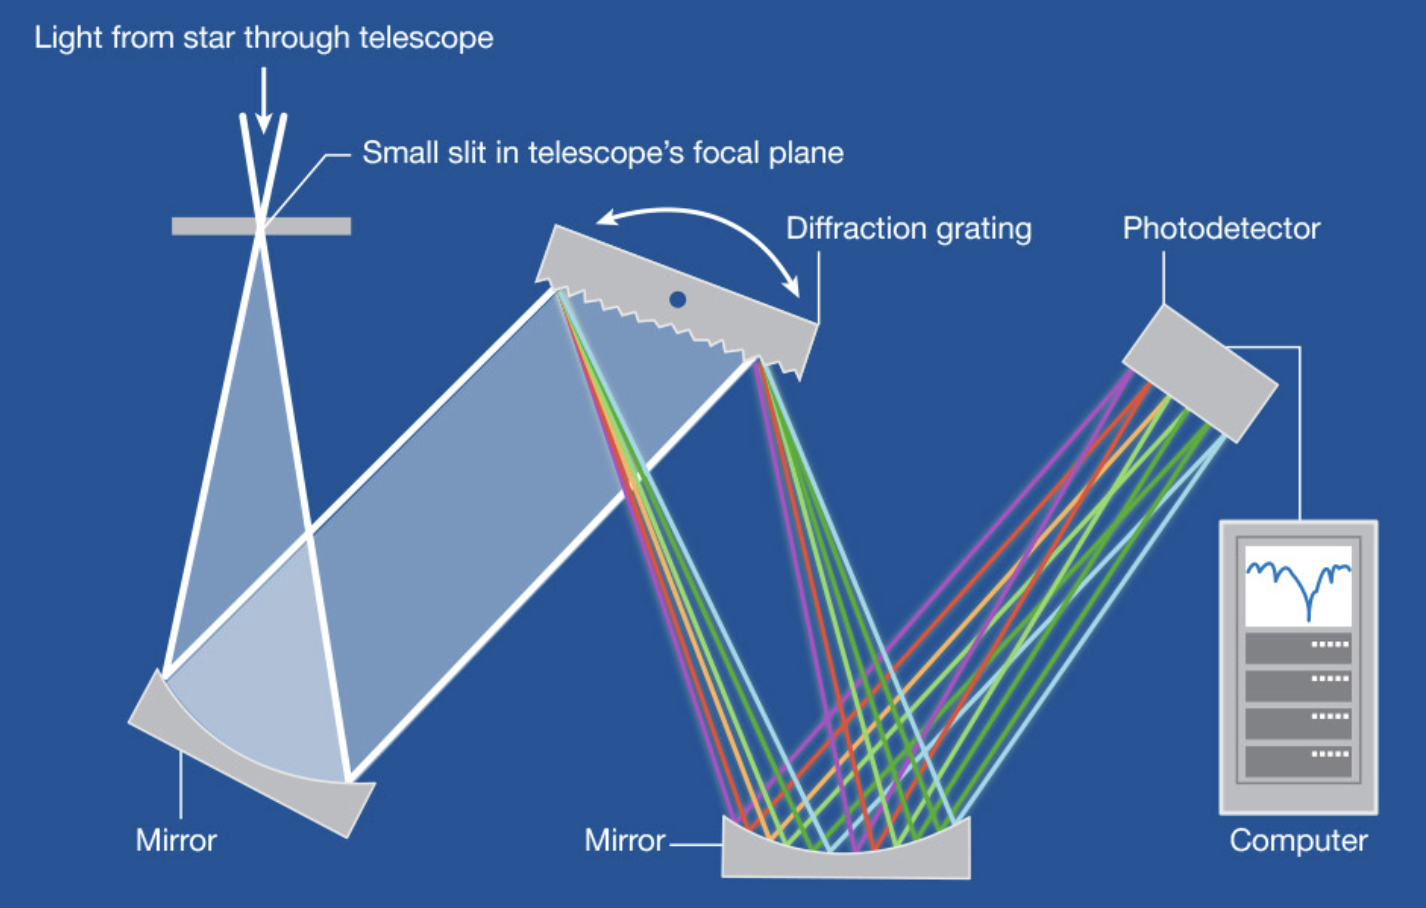
\includegraphics[width=0.65\textwidth]{spectroscopy.png}
    \caption{Light from a star passes through a telescope and gets split into many wavelengths before it gets analyzed on a computer. (Pasco)}
    \label{fig:spectro}
\end{figure}

\noindent Another important quantity for estimating star size is \textbf{luminosity}. Luminosity refers to the total amount of energy emitted by a star per unit of time. The larger the star, the more surface area it has available to emit light and heat, resulting in a higher luminosity. Conversely, a smaller star will have a lower luminosity because it has less surface area. The luminosity of a star can be measured (by various methods, including spectroscopy). 
\\\\
Luminosity, temperature, and size for a star are all related quantities. Astronomers call this well-studied relationship the \textbf{Stefan-Boltzmann} law. The equation looks like this:
\begin{equation}
    L = 4 \pi R^2 \sigma T^4
\end{equation}
This equation looks a bit complicated, but the main point is that if you know two of the quantities, say luminosity $L$ and temperature $T$, you can find the other one, in this case the size $R$! Don't pay too much attention to the symbol $\sigma$; it just represents a constant called the Stefan-Boltzmann constant and always has the same value.

\begin{figure}[htbp]
    \centering
    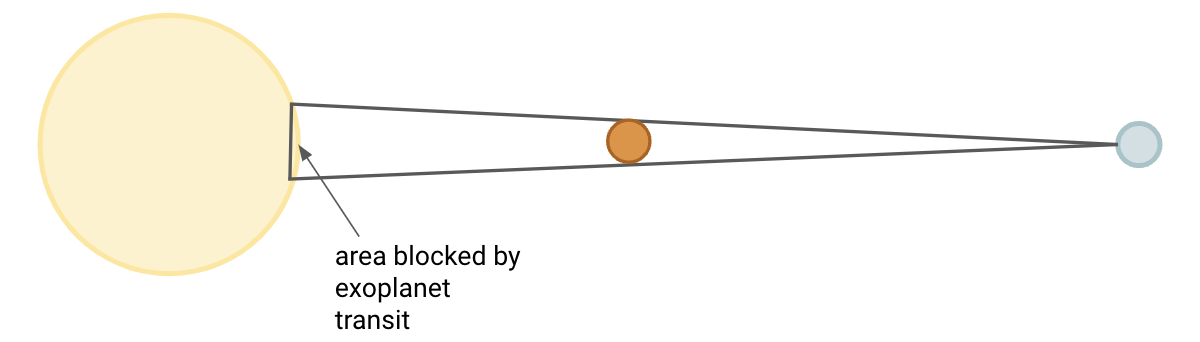
\includegraphics[width=0.6\textwidth]{exo_area1.png}
    \caption{An orbiting exoplanet passes between its host star and the observer, blocking some of the total light the observer collects.}
    \label{fig:area1}
\end{figure}

\noindent You may have also been wondering where the planet size equation came from in the first place. This equation is a useful approximation that considers the star and the exoplanet as two-dimensional spheres (i.e. circles!) and relates their areas to the total brightness. When an exoplanet is orbiting a star, it will eventually pass between the star and the observer like in Figure \ref{fig:area1}. 

\noindent This blocks some of the starlight that the observer can see. You can imagine that this decreases the total brightness of the system, and we talked about this during your module.
\\\\
\noindent On a plot of total brightness, there is a decrease when the exoplanet crosses in front of the star. If we estimate both the star and the exoplanet as circles, from the observers perspective, we can calculate the amount of \textbf{area} the exoplanet blocks. As a reminder, the area of a circle can be calculated as
\begin{equation}
    A = \pi R^2
\end{equation}
\noindent where $R$ is the radius of the circle. For the star and the exoplanet, we have
\begin{equation}
    A_{\text{planet}} = \pi R_{\text{planet}}^2
\end{equation}
\begin{equation}
    A_* = \pi R_*^2
\end{equation}

\noindent Dividing these two tells us how much of the star gets covered by the exoplanet - which is also how much the brightness plot dips by. So, 
\begin{equation}
    \text{depth} = \frac{A_{\text{planet}}}{A_*} = \frac{\pi R_{\text{planet}}^2}{\pi R_*^2}.
\end{equation}

\begin{figure}[h]
    \centering
    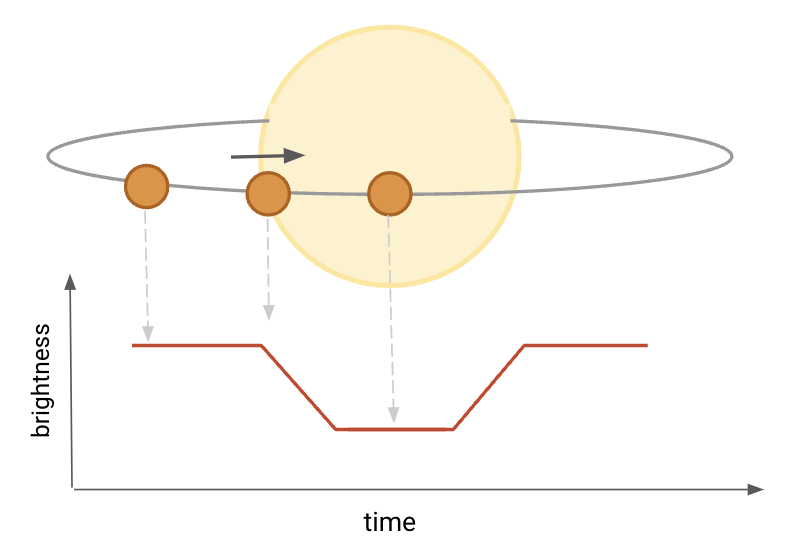
\includegraphics[width=0.5\textwidth]{exo_area2.png}
    \caption{When the exoplanet passes in front of the star, the plot of total brightness dips down an amount proportional to the area of the exoplanet.}
    \label{fig:area1}
\end{figure}

\noindent Now, we know the transit depth because it can be measured from the data. We also know the size of the star, because astronomers provide that information in the exoplanet database after they perform spectroscopy and calculations involving temperature and luminosity. From our equation, if we cancel out the $\pi$ and rearrange the equation to find the planet radius, we are left with 
\begin{equation}
    R_{\text{planet}} = R_{*} \sqrt{\text{depth}},
\end{equation}
just like in the notebook! With some algebra and approximations, we have shown where the equation that calculates the size of the exoplanet comes from.

\section{LIGO Data Processing}
\label{a:sigproc}
LIGO collects gravitational wave strain data that scientists use to learn about astrophysical sources like binary black hole mergers. However, the data collected by the detector is not immediately a perfect signal that scientists can use - they must first perform some \textbf{signal processing} to transform the raw data into data that can be used for science purposes. In order to understand gravitational wave signal processing, it is useful to draw a comparison to sound.
\\\\
\noindent Both gravitational waves and sound are waves that propagate through a medium. Sound waves travel through a medium like air or water, while gravitational waves travel through the fabric of spacetime itself. In both cases, we use specialized instruments to detect and analyze the waves. For sound, we have devices like microphones that convert sound waves into electrical signals. Similarly, we have gravitational wave detectors like LIGO that convert the waves into measurable signals.
\\\\
\noindent In any situation where a person wants to analyze waves, some kind of signal processing is required to enhance the quality of signals and make sense of complex data. In audio processing, we often manipulate and examine sound signals to extract useful information. This includes tasks like filtering, amplifying, and analyzing the frequency content of the sound. Likewise, in gravitational wave signal processing, scientists apply various techniques to enhance and analyze the signals received from detectors. This involves filtering out noise, enhancing the weak gravitational wave signals, and extracting information from the waveforms.
\\\\
\noindent As we mentioned, it is useful to analyze the frequency content of a sound wave. Sound waves have a range of frequencies that determine their pitch or tone. Humans can perceive audio sound within a specific frequency range, typically between 20 Hz to 20,000 Hz, where Hertz (Hz) is a standard unit of frequency that measures how many cycles of the wave occur per second. Take a look at Figure \ref{fig:freq_ear} for some sound ranges the human ear can typically hear. For example, the frequency that corresponds to the musical note A is 440 Hz - so that sound wave that creates the musician's A has 440 cycles each second! Each frequency corresponds to different pitches. This is an example of how frequency content of a wave corresponds to useful information. Gravitational waves also have a frequency spectrum. However, the frequencies involved are much lower. Gravitational waves from astrophysical sources can span an even wider range of frequencies than those of sounds humans can hear, from millihertz (about 0.001 Hz) to kilohertz (1000 Hz).


\begin{figure}[h]
    \centering
    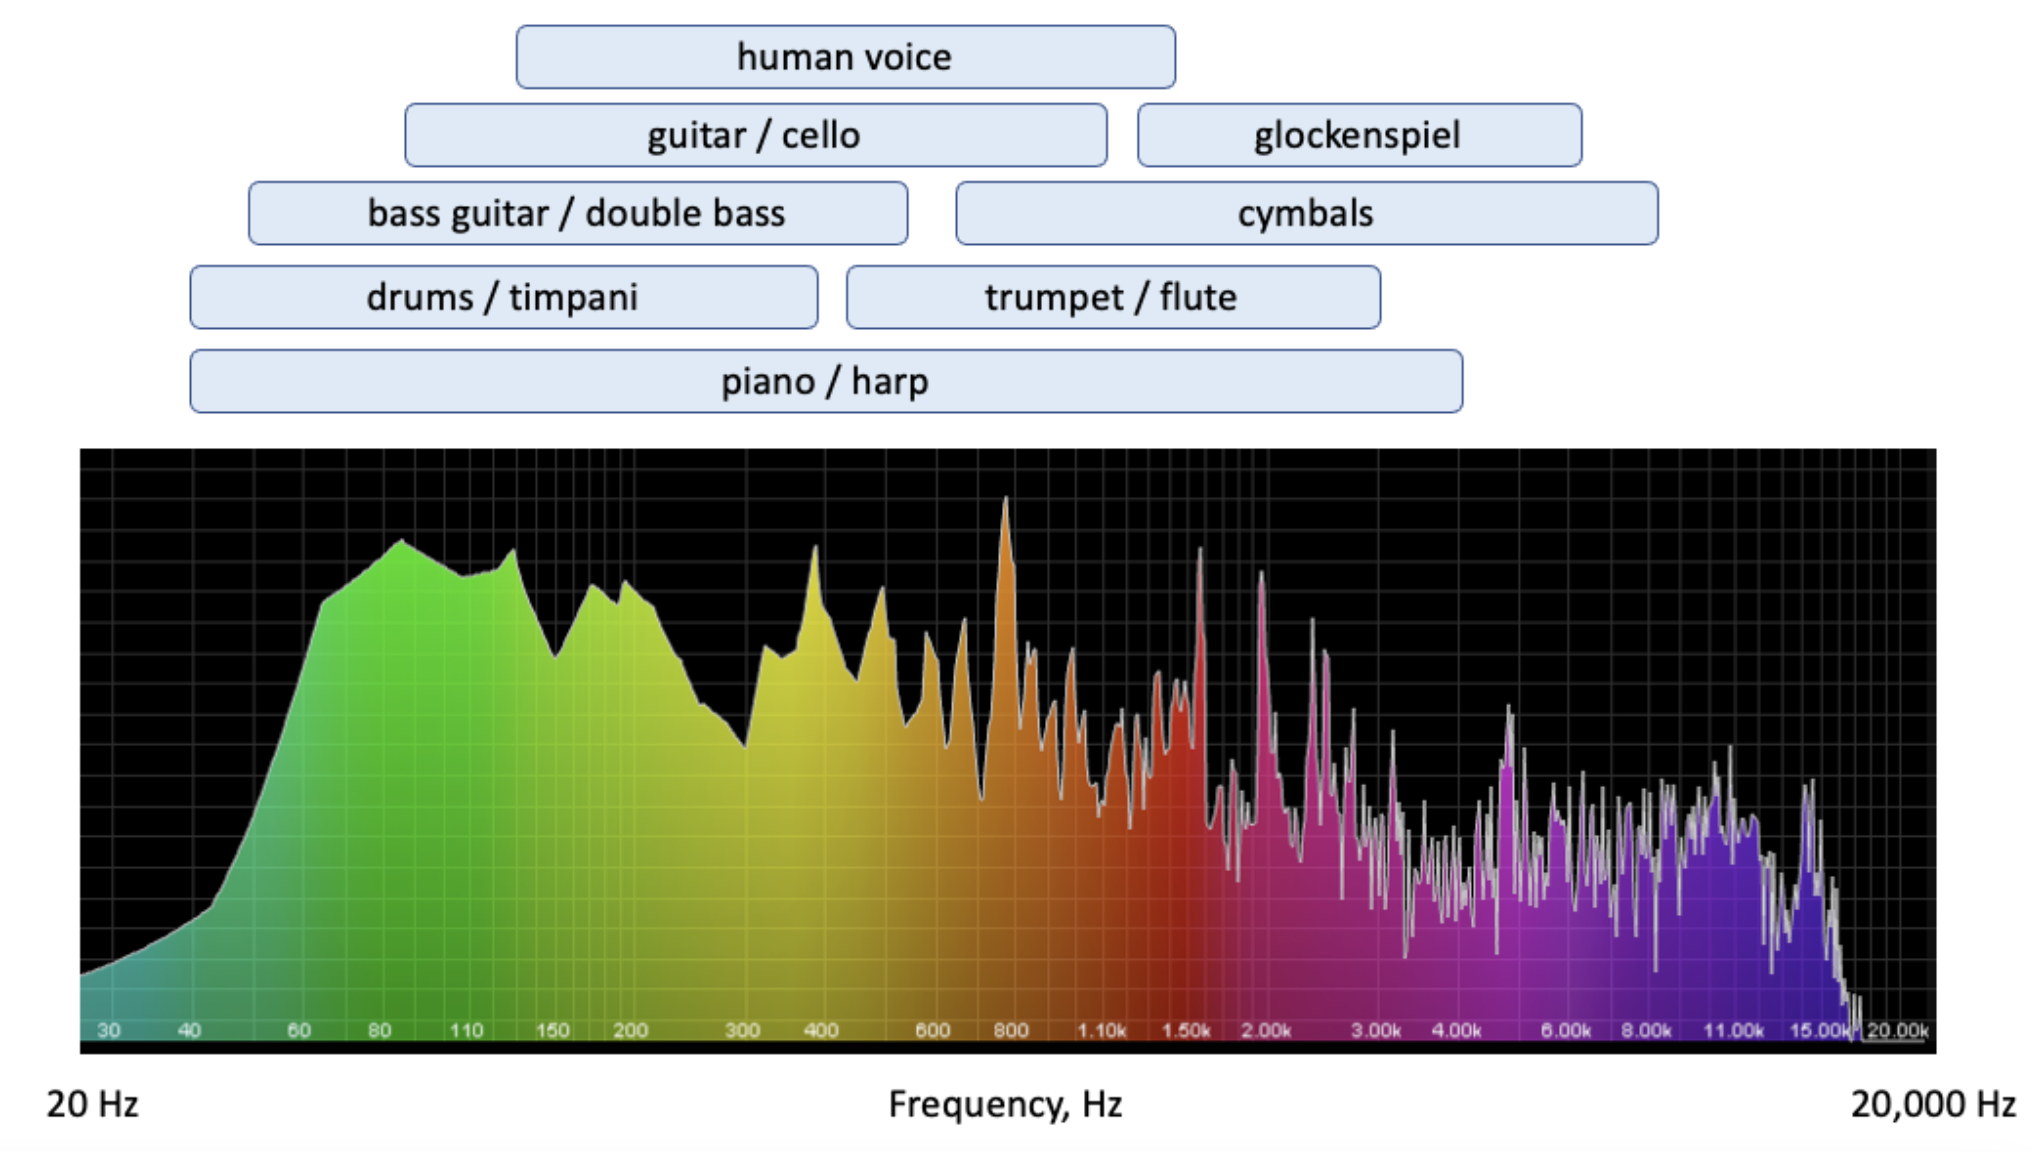
\includegraphics[width=0.65\textwidth]{freq_spec.png}
    \caption{The audio range perceived humans is on average about 20 Hz to 20,000 Hz. Here is an example of the frequency ranges covered by some instruments that are within the typical range of a human. (iDrumTune)}
    \label{fig:freq_ear}
\end{figure}

Both sound and gravitational waves carry information about their sources. In the case of sound, we can identify different musical instruments or spoken words based on the unique patterns in the sound waves. Just as for sound, scientists can extract valuable information about astrophysical phenomena from gravitational waves. The waveform of a gravitational wave can reveal details about the masses, velocities, and distances of the objects that produced it. 
\\\\
\noindent In both sound and gravitational wave signal processing, minimizing \textbf{noise} is crucial for accurate analysis and interpretation of the desired signals. In general, noise is classified as any unwanted signals or disturbances that the detector may identify, but are not signal scientists are hoping to study. Sources of noise for sound are things like background chatter or interference. For gravitational waves, noise can come from seismic events (earthquakes, human activities, etc.) or instrument effects, among many others! Techniques and strategies are employed to mitigate noise and enhance the signal-to-noise ratio, enabling scientists to extract meaningful information from the data.
\\\\
\noindent Scientists extensively study the sources of noise to develop sophisticated models and strategies for noise reduction. They employ advanced algorithms and statistical methods to identify and remove noise components from the gravitational wave data. The final result of gravitational wave data processing is a representation of \textit{only} the signal. Then, scientists can proceed with fitting signal templates to the real data to learn more about the source, just as you did in your module! 
\\\\
\noindent If you are interested in seeing what the raw data looked like for gravitational wave event GW150914, the final cell of your notebook creates a plot that shows the data prior to any signal processing. To see it, remove the \texttt{\#} from the beginning of the lines that say \texttt{\#ligo\_data = loadLIGOdata()} and \texttt{\#plotLIGOdata(ligo\_data)}. Run the cell. The plot created by this cell shows the detector data before any nice signal processing is performed. For a more detailed, hands-on example, see the official \href{https://gwfilter.streamlit.app/}{LIGO signal processing tutorial}.

% POINT: get from raw data to something that looks like a signal? Basically a signal processing motivation/discussion
% \\\\
% - make comparison signals/frequencies to sound analogy \\
% - signals composed of multiple frequencies \\
% - time domain vs. freq domain \\
% - brief discussion of noise and sources \\
% - run last bonus cell in NB to see raw data
% \noindent Any signal can be represented by a series of measurements over time, or by its frequency content. Typically, multiple frequencies are added together to make a signal, and it can be difficult to distinguish \textit{which} frequencies contribute how much \textit{amplitude} to the signal. Signals are also usually obscured by noisy data. Scientists need ways to disentangle nice signals from the noise.
% \\\\
% \noindent Broadly, LIGO collects strain time series data. This means that for each time step, the strain is recorded. Strain $h$ is defined as
% \begin{equation}
%     h = \frac{\Delta x}{L}
% \end{equation}
% where $\Delta x$ is the amount of change in length of the detector arm caused by a passing gravitational wave and $L$ is the total, original length of the arm when a gravitational wave is not passing. Strain can be thought of as the strength of the signal, and when one arm is being stretched, the other is being compressed. See Figure \ref{fig:ligo} for a reminder about how LIGO works. 
% \\\\
% \noindent A passing gravitational wave causes a laser interference pattern to appear on the photodetector. Terabytes of this kind of data are generated each day during observing runs. The changing patterns of flickering light allow scientists to determine how the arms of the detector must have been changed in order to have generated the observed pattern. The patterns tell us both how much the arms changed length during the wave's journey as well as the how quickly (the frequency) the arms changed lengths.
% \\\\
% The time series used in your example notebook contain $32$ secs of data collected around the first gravitational wave event ever detected, GW150914, which happened on September 14, 2015. The first data processing step is checking that you are only using valid data. Sometimes LIGO data may contain samples that are invalid. This can happen when the detector had a malfunction, experienced calibration errors, or had data acquisition problems. LIGO implements data quality checks to ensure the data is valid to be used for science purposes. If the data has some invalid values, scientists need to write code to loop over only the good sections of data to use for their research.
% \\\\
% \noindent Nosiy data is another thing that complicates the study of these signals. Additionally, there are different categories of noise. They must be addressed as you begin to analyze a signal. One kind of noise is called \textbf{white noise}. This noise which has about the same amplitude at all frequencies. \kw{Plots of white noise in both time and freq domain?} Red noise is another type of noise, which is stronger at lower frequencies. For LIGO, seismic fluctuations contribute noise at lower frequencies. However, the gravitational wave events LIGO searches for occur at higher frequencies.
% \\\\
% \noindent When scientists look at the raw data from the LIGO detectors, it does not obviously look like a signal. The data is pretty noisy! \kw{figure} We need a way to \kw{remove} the noise from the data so that we can do science with the signal itself. The first step is to attempt to \textbf{filter} out the noise we know is contributing at low frequencies. To do this, a \textbf{high pass} filter is applied to the data. The name ``high pass" comes from the fact that the filter allows the higher frequencies to pass through, filtering out the lower frequencies. This high pass filter is applied up to a certain frequency called the \textbf{cutoff} frequency. \kw{Describe making ASD and determining high/low cutoffs?}
% \\\\
% \noindent It is also common to perform a process called \textbf{whitening} as a first step in data processing. This suppresses the extra noise at low frequencies and at the spectral lines so that we can better see weak signals. Whitening is performed by re-weighting all the data so ... found at all frequencies. Then, frequencies that contain part of the signal will be louder than frequencies that only contain noise. The data is now in units of how much variation from the mean of the data is present at each time step.

\section{Lensing in Images}
\label{a:lensing}

Gravitational lensing occurs when a massive celestial body — such as a galaxy cluster — causes a sufficient curvature of spacetime for the path of light around it to be visibly bent, as if by a lens. The body causing the light to curve is accordingly called a gravitational lens. Read more about gravitational lensing \href{https://esahubble.org/wordbank/gravitational-lensing/}{here} and \href{https://esahubble.org/science/gravitational_lensing/}{here}!


\begin{figure}[h]
    \centering
    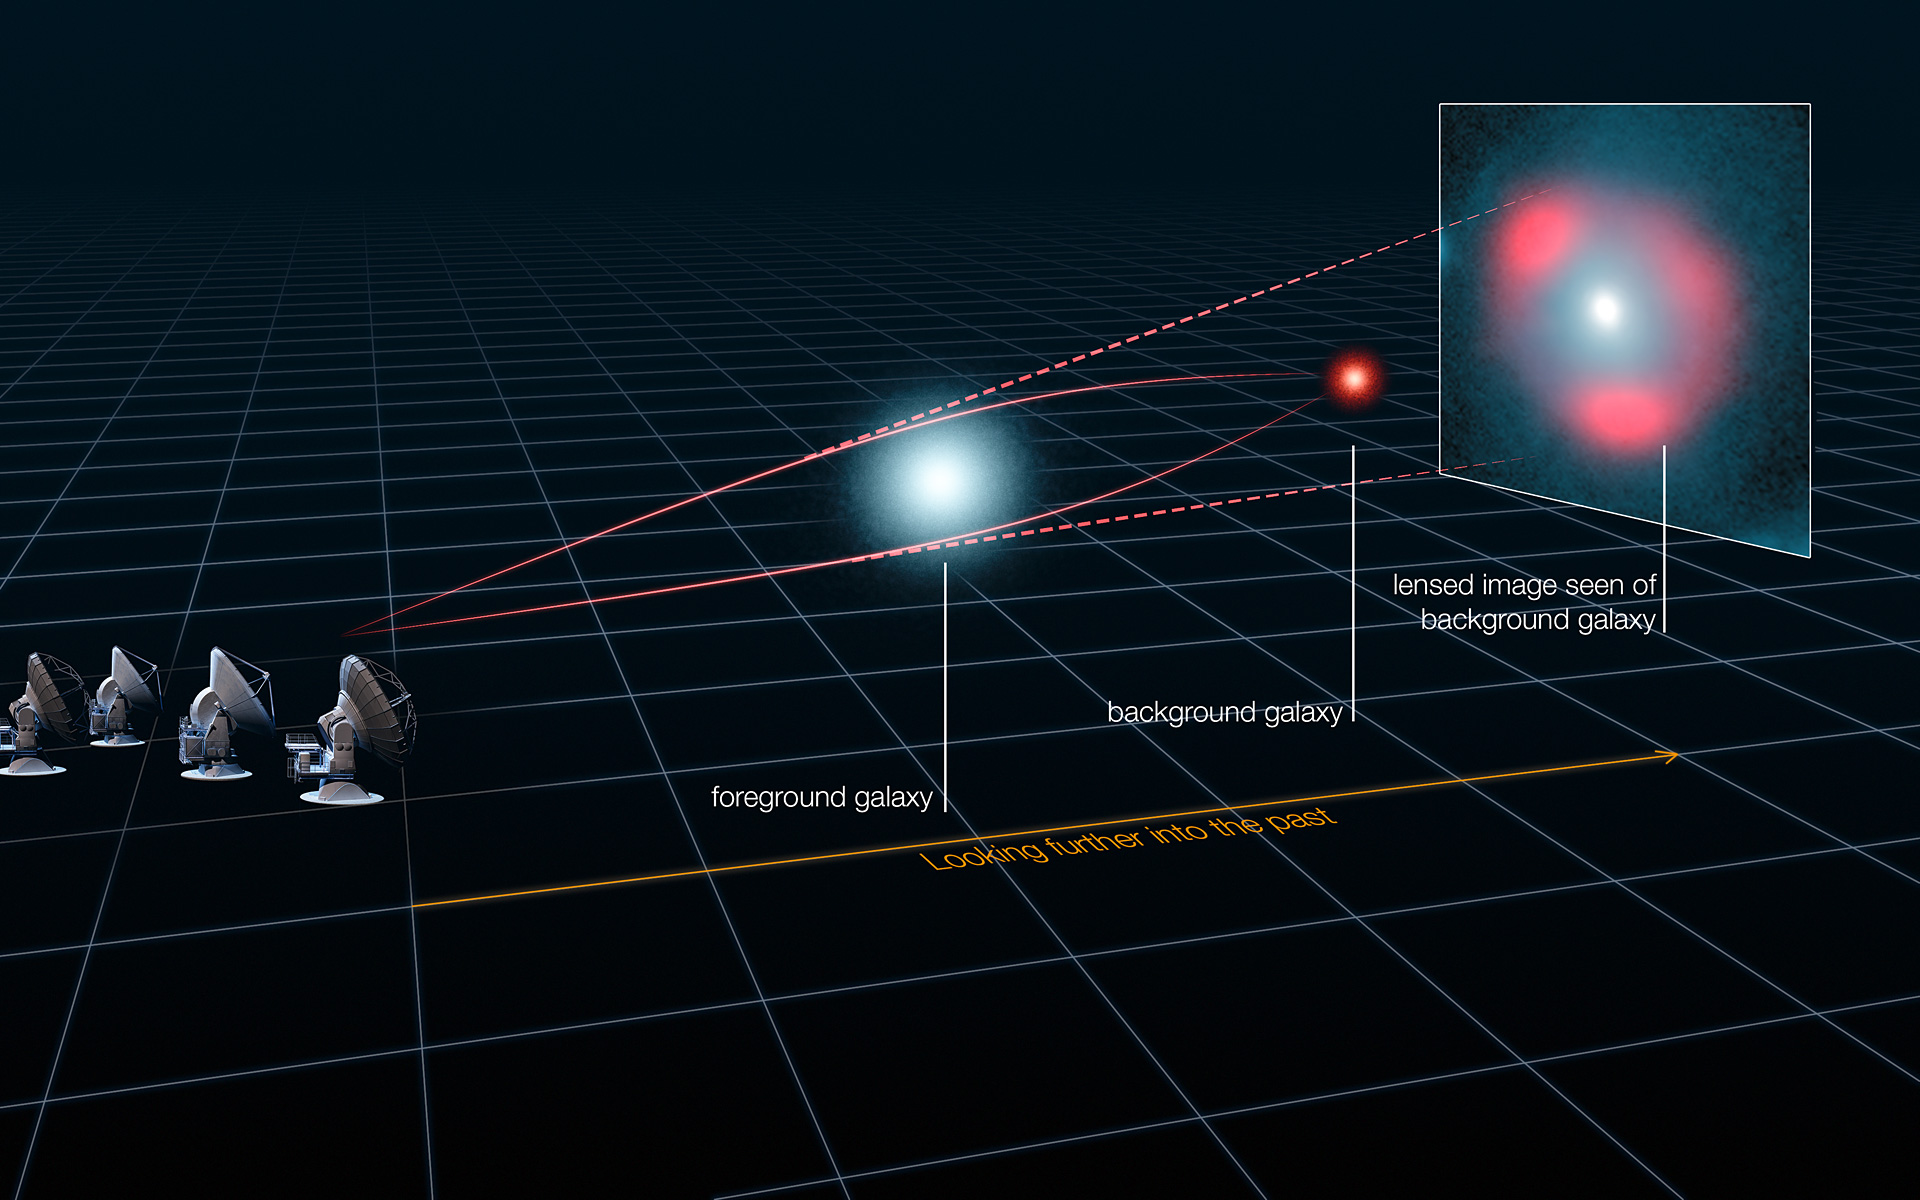
\includegraphics[width=0.75\textwidth]{lensing.jpeg}
    \caption{A foreground galaxy causes light from the background galaxy, the one that is being observed) to get bent and distorted. (ALMA)}
    \label{fig:lensing}
\end{figure}

\end{document}
